\documentclass{article}

%% BEGIN {Luke's Macros}
%%
\newif\ifdraft
\drafttrue %% To hide all comments and highlighting, just comment this line out 

\ifdraft
\usepackage[draft]{commenting}
\else
\usepackage[nompar]{commenting}
\fi

\declareauthor{lo}{L}{red}
\authorcommand{lo}{comment}

\declareauthor{akr}{A}{blue}
\authorcommand{akr}{comment}
\setdefaultauthor{akr}

\makeatletter
\renewcommand{\comm@todo@mpar}[1]{}
\makeatother

\def\divider{%
  \leavevmode\leaders\hrule height 0.6ex depth \dimexpr0.4pt-0.6ex\hfill%
  \kern0pt%
}
\newcommand{\ONGOING}[1]{%
  \draftpar\comment*{\divider\MakeUppercase{Ongoing~#1}\divider}\draftpar%
}

\renewcommand{\OpenCommentBraket}{$\lceil$}
\renewcommand{\ClosedCommentBraket}{$\rfloor$}
\usepackage{calculation}
\usepackage{graphicx}

\usepackage[square]{natbib}
\setcitestyle{aysep={}}

\definecolor{oxblue}{RGB}{0,33,71}
\definecolor{oxgold}{HTML}{a0630a}
\usepackage[final,
bookmarks,
bookmarksopen,
colorlinks,
final,
linkcolor=red,
citecolor=oxgold,
pdfstartview=FitH ]{hyperref}

\usepackage{amsmath} % cleveref must be loaded afer amsmath
\usepackage{cleveref}
\Crefname{theorem}{Theorem}{Theorems}
\Crefname{corollary}{Corollary}{Corollary}
\crefname{proposition}{Proposition}{Propositions}
\Crefname{claim}{Claim}{Claims}
\Crefname{definition}{Definition}{Definitions}
\Crefname{fact}{Fact}{Facts}
\Crefname{conj}{Conjecture}{Conjectures}
\Crefname{example}{Example}{Examples}
\Crefname{remark}{Remark}{Remarks}
\Crefname{convention}{Convention}{Conventions}
\Crefname{lemma}{Lemma}{Lemmas}
\Crefname{assumption}{Assumption}{Assumptions}
\Crefname{section}{Section}{Sections}
\Crefname{appendix}{Appendix}{Appendices}
\Crefname{figure}{Figure}{Figures}
%\Crefname{equation}{Eq.}{Equations}

% \addtotheorempostheadhook[theorem]{\crefalias{thmlisti}{theorem}}
% \addtotheorempostheadhook[lemma]{\crefalias{thmlisti}{lemma}}
% \addtotheorempostheadhook[proposition]{\crefalias{thmlisti}{proposition}}
% \addtotheorempostheadhook[corollary]{\crefalias{thmlisti}{corollary}}
% \addtotheorempostheadhook[claim]{\crefalias{thmlisti}{claim}}
% \addtotheorempostheadhook[fact]{\crefalias{thmlisti}{fact}}
% \addtotheorempostheadhook[example]{\crefalias{thmlisti}{example}}
% \addtotheorempostheadhook[definition]{\crefalias{thmlisti}{definition}}
% \addtotheorempostheadhook[remark]{\crefalias{thmlisti}{remark}}
% \addtotheorempostheadhook[assumption]{\crefalias{thmlisti}{assumption}}

\newcommand{\Real}{\mathbb{R}}
\newcommand{\nnReal}{\mathbb{R}_{{\geq}0}}
\newcommand{\pReal}{\mathbb{R}_{{>}0}}

\newcommand\expect[1]{\mathbb{E}[#1]}
\newcommand\set[1]{\{#1\}}
\newcommand\dif{\mathrm{d}}
\newcommand\calF{\mathcal{F}}
\newcommand\calI{\mathcal{I}}
\newcommand\Leb{\mathrm{Leb}}
\newcommand\ndraw[2]{\#\mathrm{draw}_{#1}(#2)}

\makeatletter
\newcommand{\dotDelta}{{\vphantom{\Delta}\mathpalette\d@tD@lta\relax}}
\newcommand{\d@tD@lta}[2]{%
  \ooalign{\hidewidth$\m@th#1\mkern-1mu\cdot$\hidewidth\cr$\m@th#1\Delta$\cr}%
}

%\usepackage[bbgreekl]{mathbbol} %for \bblambda
%%
%% END {Luke's Macros}

\usepackage{amsfonts}
\usepackage{amsthm}
\usepackage{amssymb}
\usepackage{verbatim}
\newcommand{\tY}{\textsf{Y}}
\newcommand{\tif}[3]{\textsf{if }#1\textsf{ then }#2\textsf{ else }#3}
\newcommand{\tsample}{\textsf{sample}}
\newcommand{\tscore}{\textsf{score}}
\DeclareMathOperator{\red}{red}
\DeclareMathOperator{\nnext}{next}


\usepackage{amsthm}
\theoremstyle{definition}
\newtheorem{definition}{Definition}
\newtheorem{example}{Example}

\theoremstyle{lemma}
\newtheorem{lemma}{Lemma}
\newtheorem{theorem}{Theorem}
\newtheorem{corollary}{Corollary}
\newtheorem{conjecture}{Conjecture}

\theoremstyle{remark}
\newtheorem*{remark}{Remark}

\title{Supermartingales and Termination Analysis of Statistical PCF}

\begin{document}

\maketitle

\lo{Tentative title}

\begin{abstract}
\lo{TODO}
\end{abstract}

\iffalse
\akr{Following your suggestion, I will be providing a criterion for termination of programs in PPCF \citep{DBLP:journals/pacmpl/EhrhardPT18} based on ranking supermartingales. 
As it's more convenient for this proof, a sampling-based semantics \lo{You need to provide reference(s) for sampling-based semantics.} will be used instead of the original distributional semantics. 
I assume some roughly applicable equivalence is proven somewhere, but it doesn't seem that hard anyway.}
\lo{Why not provide a proof as an appendix?}
\fi

\tableofcontents

Various theorems about probabilistic programs rely on the assumption that the program terminates almost surely. Proof rules based on relating the program state to supermartingales already exist for first-order imperative programs \citep{DBLP:journals/pacmpl/McIverMKK18}. This paper's contribution is to extend this method to a higher-order setting.

\section{Statistical PCF}

\subsection{Syntax of SPCF}

The language SPCF is a simply-typed lambda calculus with sampling of real numbers from $[0,1]$ and unbounded scoring, following \cite{MakOP20b}. Types and terms are defined as follows, where $r$ is a real, $x$ is a variable, $f : \mathbb{R}^n \to \mathbb{R}$ is any measurable function and $\Gamma$ is an environment:
\begin{align*}
  & \text{types } A, B ::= \textsf{R}  \mid  A \to B \\
  & \text{values } v ::= \lambda x.s  \mid  \underline{r} \\
  & \text{terms } s, t ::= v  \mid  x  \mid  t_1 t_2  \mid  \underline{f}(s_1,\dots ,s_n)  \mid  \tY s  \mid  \tif{s < 0}{t_1}{t_2}  \mid  \tsample  \mid  \tscore(s)
\end{align*}
\begin{align*}
  \frac{}{\Gamma ; x:A \vdash x:A} \qquad
  \frac{\Gamma ; x:A \vdash s : B}{\Gamma \vdash \lambda x.s : A \to B} \qquad
  \frac{}{\underline{r} : \textsf{R}} \qquad
  \frac{\Gamma \vdash s:A \to B \quad \Gamma \vdash t : A}{\Gamma \vdash s \, t : B} \\ \\
  \frac{\Gamma \vdash s_1:\textsf{R} \dots \Gamma \vdash s_n:\textsf{R}}{\Gamma \vdash \underline{f}(s_1,\dots,s_n) : \textsf{R}} \ f : \mathbb{R}^n \to \mathbb{R} \qquad
  \frac{\Gamma \vdash s : (A \to B) \to (A \to B)}{\Gamma \vdash \tY s : (A \to B)} \\ \\
  \frac{\Gamma \vdash c : \textsf{R} \quad \Gamma \vdash s_1 : A \quad \Gamma \vdash s_2 : A}{\Gamma \vdash \tif{c < 0}{s_1}{s_2} : A} \qquad
  \frac{}{\Gamma \vdash \tsample : \textsf{R}} \qquad
  \frac{\Gamma \vdash s : \textsf{R}}{\Gamma \vdash \tscore (s) : \textsf{R}}
\end{align*}

The set of all terms is denoted $\Lambda$, and the set of closed terms is denoted $\Lambda^0$.

\paragraph{}
To define the reduction relation, let evaluation contexts be of the form:
\begin{align*}
  E ::= & \, [\,] \mid E t \mid v E \mid \underline{f}(r_1,\dots ,r_{k-1}, E, s_{k+1}, \dots, s_n) \\ & \mid \tY E \mid \tif{E<0}{s_1}{s_2} \mid \tscore (E)
\end{align*}
then a term reduces if it is formed by substituting a redex in a context i.e.
\begin{align*}
  E[(\lambda x.s) v] & \to E[s[v/x]] \\
  E[\underline f (\underline r_1, \dots , \underline r_n)] & \to E[\underline{f(r_1,\dots,r_n)}] \\
  E[\tY \lambda x. s] & \to E[\lambda z. s[(\tY \lambda x. s)/x] z] \text{ where $z$ is not free in $s$}\\
  E[\tif{\underline r < 0}{s_1}{s_2}] & \to E[s_1] \text{ where }r < 0 \\
  E[\tif{\underline r < 0}{s_1}{s_2}] & \to E[s_2] \text{ where }r \geq 0 \\
  E[\tsample] & \to E[\underline r] \text{ where } r \in [0,1] \\
  E[\tscore(\underline r)] & \to E[\underline r].
\end{align*}
\changed[lo]{We write $\to^\ast$ for the reflexive, transitive closure of $\to$.}
\lo{The $\tscore$ rule should have a side condition: if $r > 0$.}

Every closed well-typed term either is a value or reduces to another term.


\subsection{Sampling semantics}
This version of the reduction relation allows $\tsample$ to reduce to any number in $[0,1]$. To more precisely specify the probabilities, an additional argument is needed to determine the outcome of random samples. Let $ I = [0,1] \subset \mathbb{R} $, and let $S = I^{\mathbb{N}}$, with the \changed[lo]{Borel $\sigma$-algebra $\calF$} and the probability measure, denoted $\mu$, given by the limit of $1 \gets I \gets I^2 \gets \cdots$, where the maps are the projections that ignore the last element. Equivalently, a basis of measurable sets is $\prod_{i=0}^\infty X_i$ where $X_i$ are all Borel and all but finitely many are $I$, and $\mu (\prod_{i=0}^\infty X_i) = \prod_{i=0}^\infty \Leb(X_i)$.
The maps $\pi_h:S \to I, \; \pi_t:S \to S$ popping the first element are then measurable.
\changed[lo]{Following \cite{DBLP:conf/esop/CulpepperC17}, we call the probability space $(S, \calF, \mu)$ the \emph{entropy space}.}

The $\sigma$-algebra and measure on $\Lambda$ are defined by considering it as a disjoint union of equivalence classes under replacing all the real constants by a placeholder, where the measure on each class is that of $\mathbb{R}^n$, where $n$ is the number of real constants.
\changed[lo]{Precisely, following \cite{DBLP:conf/icfp/BorgstromLGS16},
we view $\Lambda$ as $\bigcup_{m\in\omega} \big(\mathsf{Sk}_m \times \Real^m \big)$,
where $\mathsf{Sk}_m$ is the set of SPCF terms with exactly $m$ place-holders (a.k.a.~\emph{skeleton terms}) for numerals.
Thus identified, we give $\Lambda$ the countable disjoint union topology of the product topology of the discrete topology on $\mathsf{Sk}_m$ and the standard topology on $\Real^m$.
Note that the connected components of $\Lambda$ have the form $\{M\} \times \Real^m$, with $M$ ranging over $\mathsf{Sk}_m$, and $m$ over $\omega$. 
We fix the Borel algebra of this topology to be the $\sigma$-algebra on $\Lambda$.}

The one-step reduction is given by the function $\red : \Lambda^0 \times S \to \Lambda^0 \times S$ where
\begin{equation}
\red(M,s) = \left\{
    \begin{array}{ll}
        (E[N],s) & \text{if } M = E[R], R \to N \text{ and } R \neq \tsample \\
        (E[\underline{\pi_h(s)}],\pi_t(s)) & \text{if } M = E[\tsample] \\
        (M,s) & \text{if } M \text{ is a value}
    \end{array} \right .
\end{equation}
\lo{Both $\to$ and $\red$ are called reduction relation.}

The result after $n$ steps is then simply $\red^n(M,s) = \overbrace{\red(...\red(}^n M,s)...)$, and the limit $\red^\infty$ can then be defined as a partial function as $\lim_{n \to \infty} \red^n(M,s)$ whenever that sequence becomes constant by reaching a value. A term $M$ terminates for a sample sequence $s$ if the limit $\red^\infty(M,s)$ is defined.

The reduction function is measurable, and the set of values is measurable, therefore the set of $s$ such that $M$ terminates at $s$ within $n$ steps is measurable for any $n$, therefore $\{s \mid M \text{ terminates at } s \}$ is measurable. A term $M$ is said to terminate almost surely if $\mu(\{s \mid M \text{ terminates at } s\}) = 1$.

\lo{Alternatively, define the \emph{runtime of $M$} to be the random variable 
\[
T_M(s) := 
\begin{cases}
\min \set{n \mid \pi_0(\red^n(M, s)) \textrm{ is a value}} & \hbox{if $\red^\infty(M,s)$ is defined}\\
\infty & \hbox{otherwise}
\end{cases}
\]
Equivalently, we say that $M$ is \emph{almost-surely terminating} (AST) if $T_M < \infty$ a.s.; 
and $M$ is \emph{positively almost-surely terminating} (PAST) if $\expect{T_M} < \infty$.}

For example, the term 
\[
(\tY \lambda f, n: \tif{\tsample - 0.5 < 0}{n}{f (n+1)} ) \, \underline{0},
\] 
which generates a geometric distribution, terminates on the set $S \setminus [0.5,1]^\mathbb N$, which has measure 1, therefore it terminates almost surely, whereas 
\[
\tif{\tsample - 0.5 < 0}{\underline 0}{(\tY \lambda x. x) \underline 0},
\] 
which terminates on the set $\pi_h^{-1}[[0,0.5]]$, has probability 0.5 of failing to terminate.

\paragraph{}
Note that the requirement that $M$ be closed is not important for the proofs of the theorems, but is simply required to ensure that $M$ reaches a value, rather than a general normal form like $x \, y$.

\paragraph{}
This definition of almost sure termination is equivalent to that given in \citep{MakOP20b}, although the program semantics is stated in a slightly different way. In particular, the argument to $\tscore$ is not relevant to termination (except for the possibility that its argument's evaluation wouldn't terminate).

\lo{Your operational semantics does not maintain a record of the current weight of the reduction.
A.s.~termination does depend on $\tscore$: see \cite[\S 4.3]{DBLP:journals/corr/abs-2004-03924}\footnote{\url{https://arxiv.org/abs/2004.03924}}.
I think it important to take the behaviour of $\tscore$ into account;
you should do it as a future task.}

\section{Alternative Semantics}
\akr{This version of the semantics is much more convenient for allowing multiple different reduction orders. I don't currently have a proof of the equivalence of this with the more usual semantics. I expect that that would be somewhat complicated, but not terribly difficult. I don't know whether a semantics like this has already been defined elsewhere. I just thought I'd write it out so you can see it and in case I use it later. If I do end up actually using it I'll write it up nicer, but hopefully this is at least enough for you to understand what I mean.

Having thought a bit more about this, I realise it may not be quite right. I'll see if I can fix it later.}
\lo{I'll read this after you fix it ;-)}

When proving almost sure termination in this way \akr{I guess I should move this section somewhere later.}, it is necessary to consider which terms a given term may reduce to. Sometimes however, the reduction that the programmer has in mind may not be strictly the call-by-value order defined so far, or considering an alternative reduction order may be simpler or more intuitive.

Non-probabilistic lambda calculi generally have the Church-Rosser property, that if a term $A$ reduces to both $B_1$ and $B_2$, there is some $C$ with reduction sequences $B_1 \to^* C$ and $B_2 \to^* C$, so the reduction order mostly doesn't matter. In the probabilistic case, this may not be true, because $\beta$-reduction can duplicate $\tsample$s, so the outputs of the copies of the sample may be identical or independent, depending on whether the sample is taken before or after $\beta$-reduction. There are, however, some restricted variations on the reduction order that do not have this problem.

\paragraph{}
Even with this restriction, a sampling semantics in the style of the one already defined would not be entirely Church-Rosser, as, for example, $\red^3(\tsample - \tsample, (1,0,\dots))$ would be either $1$ or $-1$ depending on the order of evaluation of the $\tsample$s, as that determines which sample from the pre-selected sequence is used for each one. To fix this, rather than pre-selecting samples according to the order they'll be drawn in, select them according to the position in the term where they'll be used instead.

A position \akr{I'm not really sure how to phrase the citation, but this is adapted from \cite{Kennaway96infinitarylambda}.} is a finite sequence of steps into a term, defined inductively as
\begin{align*}
P ::= \cdot \mid \lambda ; P \mid @_1 ; P \mid @_2 ; P \mid \underline f_i ; P \mid \tY ; P \mid \textsf{if}_1 ; P \mid \textsf{if}_2 ; P \mid \textsf{if}_3 ; P \mid \tscore ; P.
\end{align*}
The \changed[lo]{\emph{subterm of $M$ at a position $P$}, denoted $M \mid P$,} is defined as
\begin{align*}
M \mid \cdot & = M \\
\lambda x. M \mid \lambda ; P & = M \mid P \\
M_1 M_2 \mid @_i ; P & = M_i \mid P \quad \text{for } i = 1,2 \\
\underline f(M_1,\dots,M_n) \mid \underline f_i ; P & = M_i \mid P \quad \text{for }i \leq n \\
\tY M \mid \tY ; P & = M \mid P \\
\tif{M_1 < 0}{M_2}{M_3} \mid \textsf{if}_i ; P & = M_i \mid P \quad \text{for } i = 1,2,3 \\
\tscore(M) \mid \tscore ; P & = M \mid P
\end{align*}
so that every subterm is located at a unique position, but not every position corresponds to a subterm (e.g. $x \, y \mid \lambda ; \cdot$ is undefined). A position such that $M\mid P$ does exist is said to occur in $M$. Substitution at a given position, $M[N/P]$, is defined similarly.

Two subterms $N_1$ and $N_2$ of a term $M$, corresponding to positions $P_1$ and $P_2$, can overlap in a few different ways. If $P_1$ is an initial segment (i.e.~prefix) of $P_2$ (written as $P_1 \leq P_2$), then $N_2$ is also a subterm of $N_1$. If neither $P_1 \leq P_2$ nor $P_1 \geq P_2$, the positions are said to be disjoint. This is mostly relevant in that in any substitution at some position, the subterms at all other positions are unaffected.

With this notation, a more general reduction relation $\to$ can be defined. \akr{It would almost work to have one of the neater versions of $\tY$-reduction here.}
%\lo{On first reading, I struggled to parse the following clauses.}
\changed[lo]{The binary relation $\to$ is defined by the following rules, each is conditional on a redex occuring at position $P$ in the term $M$.}
\begin{align*}
  \text{if } M \mid P = (\lambda x.s) v,\ & M \to M[s[v/x]/P] \\
  \text{if } M \mid P = \underline f (\underline r_1, \dots , \underline r_n),\ & M \to M[\underline{f(r_1,\dots,r_n)}/P] \\
  \text{if } M \mid P = \tY \lambda x. s,\ & M \to M[\lambda z. s[(\tY \lambda x. s)/x] z/P] \text{ where $z$ is not free in $s$}\\
  \text{if } M \mid P = \tif{\underline r < 0}{s_1}{s_2},\ & M \to M[s_1/P] \text{ where }r < 0 \\
  \text{if } M \mid P = \tif{\underline r < 0}{s_1}{s_2},\ & M \to M[s_2/P] \text{ where }r \geq 0 \\
  \text{if } M \mid P = \tsample & \text{ and $\lambda$ does not occur after $@_2$ or $\tY$ in $P$},\\ & M \to M[\underline r/P] \text{ where } r \in [0,1] \\
  \text{if } M \mid P = \tscore(\underline r),\ & M \to M[\underline r/P].
\end{align*}
In each of these cases, $M \mid P$ is the redex, and reduction takes place at $P$.
\lo{The definition above is clear. But as a general rule, it is good to illustrate definitions -- especially if they are genuinely new -- with an example or two.}

\paragraph{}
Labelling the pre-chosen samples by the positions in the term would also not work because in some cases, a $\tsample$ will be duplicated before being reduced, for example, in $(\lambda x. {\underline x \, 0} \, \mathbin{\underline{+}} \, {x \, \underline 0}) (\lambda y. \tsample)$, both of the $\tsample$ redexes that eventually occur originate at $@_2 ; \lambda$. It is therefore necessary to consider possible positions that may occur in other terms reachable from the original term. This is itself inadequate because some of the positions in different reachable terms need to be considered the same.

Given a closed term $M$, let $L_0(M)$ be the set of pairs, the first element of which is a reduction sequence starting at $M$, and the second of which is a position in the final term of the reduction sequence. Reduction sequences are used rather than reachable terms because if the same term is reached twice, different samples may be needed, but they will be discussed as though they were terms, by abuse of notation. \lo{Readers would benefit greatly from some examples of an $L_0(M)$-pair, and the relations $\sim_p$ and $\sim_c$, here, before the formal definitions. Explain the underlying intuition.} The relation $\sim$ is defined as the union of the symmetric relations $\sim_p$ \changed[lo]{($p$ for parent-child relationship)} and $\sim_c$ \changed[lo]{($c$ for cousin relationship)} where
\lo{As defined, $\sim_p$ is not a symmetric relation.}
\begin{enumerate}
    \item If $N$ reduces to $O$ with the redex at position $P$\lo{Do you mean: $M \to^\ast N \to O = N[\dotDelta / P]$ for some redex contraction $\Delta \to \dotDelta$}, and $Q$ is a position in $N$ disjoint from $P$, then $(N,Q) \sim_p (O,Q)$.
    
    \item If $N$ $\beta$-reduces to $O$ at position $P$, $Q$ is a position in $N \mid P;@_1;\lambda$ and $N \mid P;@_1;\lambda;Q$ is not the variable involved in the reduction, $(N,P;@_1;\lambda;Q) \sim_p (O, P;Q)$
    
    \item If $N$ $\textsf{if}$-reduces to $O$ at position $P$, with the first resp. second branch being taken, and $P;\textsf{if}_i;Q$ occurs in $N$ (where $i = 2$ resp. $3$), $(N,P;\textsf{if}_i;Q) \sim_p (O,P;Q)$
    
    \item If $N$, $O_1$ and $O_2$ match any of the following cases:
    \begin{enumerate}
        \item $N$ contains redexes at positions $P_1$ resp.~$P_2$, $O_1$ is $N$ reduced first at $P_1$
        
        \item $N \mid P = \tif{\underline r < 0}{N_1}{N_2}$, where $r < 0$ (or, respectively, $r \geq 0$), $(N_2 \text{ resp. } N_1) \mid Q$ is a redex, and $O_1$ is $N$ reduced at $P$ and $O_2$ is $N$ reduced first at $P;(\textsf{if}_3 \text{ resp. } \textsf{if}_2);Q$ then at $P$
        
        \item $N \mid P = \tif{\underline r < 0}{N_1}{N_2}$, where $r < 0$ (or, respectively, $r \geq 0$), $(N_1 \text{ resp. } N_2) \mid Q$ is a redex, and $O_1$ is $N$ reduced first at $P$ then at $P;Q$ and $O_2$ is $N$ reduced first at $P;(\textsf{if}_2 \text{ resp. } \textsf{if}_3);Q$ then at $P$
        
        \item $N \mid P = (\lambda x. A) B$, there is a redex in $A$ at position $Q$, $O_1$ is $N$ reduced first at $P$ then at $P;Q$, and $O_2$ is $N$ reduced first at $P;@_1;\lambda;Q$ then at $P$
        
        \item $N \mid P = (\lambda x. A) B$, $B \mid Q$ is a redex, $(R_i)_i$ is a list of all the positions in $A$ where $A \mid R = x$, $O_1$ is $N$ reduced first at $P ; @_2 ; Q$ then at $P$, and $O_2$ is $N$ reduced first at $P$ then at $P;R_i;Q$ for each $i$ in order.
        
        \item $N \mid P = \tY (\lambda x. A)$, $A$ reduced at $Q$ is $A'$, $(R_i)_i$ is a list of all the positions where $A' \mid R  = x$, $O_1$ is $N$ reduced first at $P;\tY;\lambda;Q$ then at $P$, and $O_2$ is $N$ reduced first at $P$ then at $P;\lambda;@_1;Q$ then at $P;\lambda;@_1;R_i;Y;\lambda;Q$ for each $i$ in order.
    \end{enumerate}
    and $O_1$ and $O_2$ are equal as terms, but with different reduction sequences (which merely requires that in cases a, c and d, if the redexes of unspecified type are $\tsample$, corresponding $\tsample$s reduce to the same numbers), $O_1'$ and $O_2'$ are the results of applying some reduction sequence to each of $O_1$ and $O_2$ (the same reductions in each case, which is always possible because they're equal terms), and $S$ is a position in $O_1'$ (or equivalently $O_2'$), then $(O_1',S) \sim_c (O_2',S)$.
\end{enumerate}

\begin{figure}
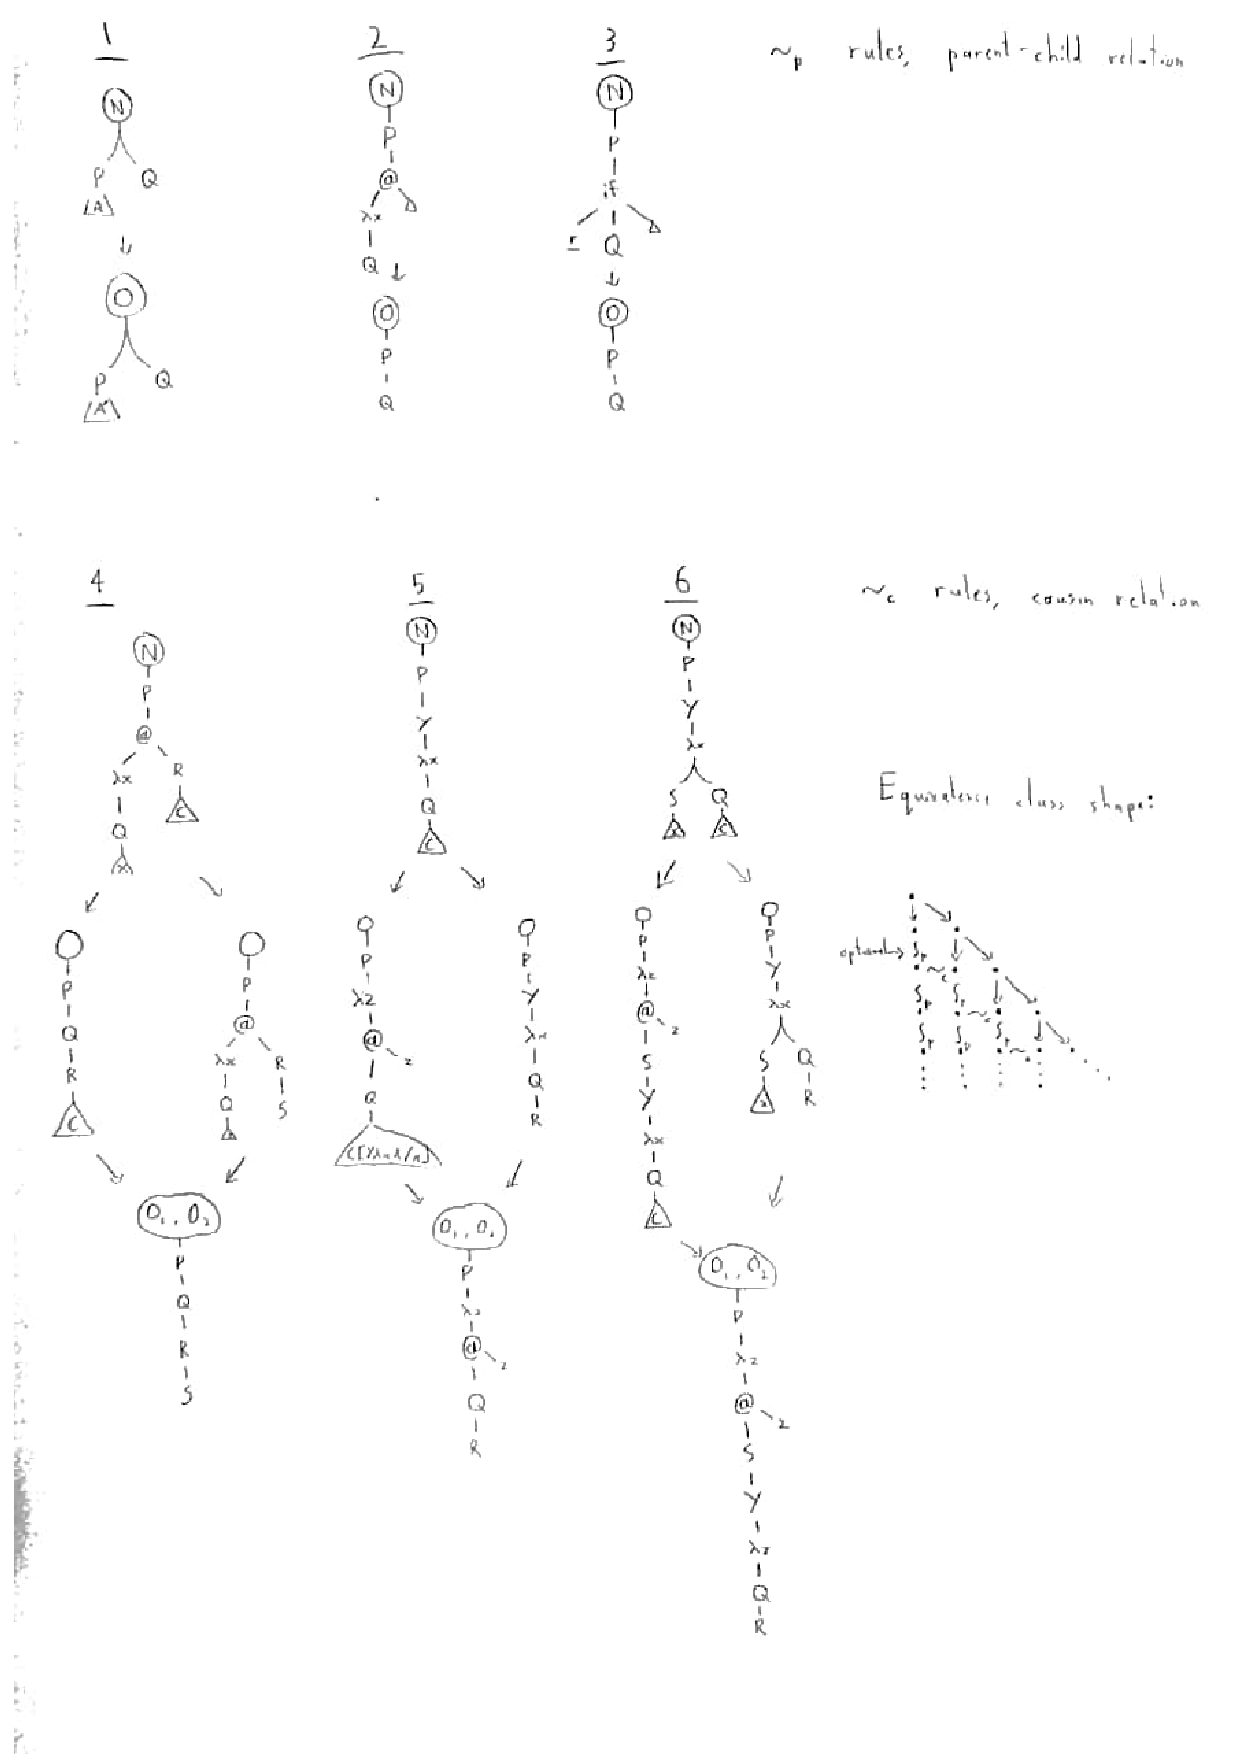
\includegraphics[height=0.9\textheight]{akr-diagram.pdf}
\caption{\label{fig:adk-diagram} Some examples of the old version of the $\sim_p$- and $\sim_c$-rules}
\end{figure}

\begin{example}
See \Cref{fig:adk-diagram} for a graphical depiction of $\sim_p$- and $\sim_c$-rules.
\end{example}

The reflexive transitive closure $\sim^*$ of this relation is used to define the set of potential positions $L(M) = L_0(M) / \sim^*$, and each equivalence class can be considered as the same position as it may occur across multiple reachable terms. If $(N,P) \sim^* (O,Q)$, then $N \mid P$ and $O \mid Q$ both have the same shape (i.e.~they're either both variables, both applications, both $\tsample$s etc.), therefore it's well-defined to talk of the set of potential positions where there is a $\tsample$, $L_s(M)$. The new sample space is then defined as $I^{L_s(M)}$, with the Borel $\sigma$-algebra and product measure.

\paragraph{}
The proofs that follow are based on a previous version of $\sim$. I intend to update them after making more progress on the antitone-strict supermartingale completeness result, but for now, here's a summary of the lemmas and theorems I intend to prove about it:
\begin{itemize}
    \item If $M \to N$, the relation $\sim_N^*$ defined on $Rch(N)$ is equal to the restriction of $\sim_M^*$ to $Rch(N)$ \lo{Define $\sim_N^*$.}
    \item Given the definition below of $\Rightarrow$, which is still applicable to this version of $\sim$, and which is the equivalent of $\red$ in this version of the semantics, $\Rightarrow$ is Church-Rosser.
    \item If $M \to N$ at $P$, no position in any term in $Rch(N)$ is related to $(M,P)$ by $\sim_M^*$, and therefore each sample is used at most once in any reduction sequence.
    \item The subprobability distribution of values obtained by reducing a term in the usual call-by-value semantics is equal to that obtained by any reduction strategy on $\Rightarrow$ (i.e.~a sub-relation of $\Rightarrow$ that is a function) (with some allowance made for the fact that some values are not normal forms of $\Rightarrow$, so the reduction strategy might overshoot the value that $\red^\infty$ reaches. I'm not quite sure what form this will take.)
    \item Similarly, the probability of termination is equal in $\red^\infty$ and any reduction strategy on $\Rightarrow$, so almost sure termination can be equivalently defined based on $\Rightarrow$.
    \item For any closed term $N$, if there is any reduction strategy for $N$ and ranking function corresponding to that reduction strategy, $N$ is AST.
    \item Corresponding sparse and antitone-strict ranking function theorems.
\end{itemize}

\paragraph{}
Before defining the new version of the reduction relation $\red$, a few lemmas about the properties of $\sim$ are necessary for it to be well-defined. Considering the set of paths through $Rch(M)$ (which we're implicitly identifying with $Rch(M)$ itself) as a tree rooted at (the trivial path at) $M$, $\sim_p$ only relates positions in child and parent terms, and $\sim_c$ only relates first cousins. Furthermore, by a case analysis on the forms of positions, the possible paths $N_1 \sim N_2 \sim \dots \sim N_n$ can be strongly restricted.

In any case, a position can be related to at most one position in each child term. Letting $P$ be the position of the redex and $Q$ the original term, this is by rule 1 if $P$ and $Q$ are disjoint, rule 2 if $P;@_1 \leq Q$ and rule 3 if $P;if_i \leq Q$. As $M$ itself has no cousins or parents, this is the only way positions in $M$ are related to others.

For any other term $N$ and position $Q$ in it, take the parent $N'$ and the position $P$ of the reduction $N' \to N$. The positions that $(N,Q)$ are related to other than those in the children of $N$ are as follows. If $Q \not \geq P$, only case 1 applies. If $Q \geq P$ and $(N,Q) \sim_p (N',Q')$ by cases 2 or 3, $Q'$ is also $\geq P$ therefore if $(N,Q)$ is also related to something by $\sim_c$, $(N',Q')$ is not related to anything in its parent. Furthermore, letting $Q = P;R$, $Q' = P;@_1;\lambda;R$ or $P;\textsf{if}_i;R$ depending on what sort of reduction $N' \to N$ was ($\beta$, $\textsf{if}$-true or $\textsf{if}$-false respectively) therefore in any case, $(N,Q)$ is related to at most one position in $N'$.

Considering now $\sim_c$, let $N'' \to N' \to N$, where the outermost of the two reductions takes place at $P$. Cases 5 and 6 can be distinguished from case 4 by whether $P;\tY$ exists in $N''$, and cases 5 and 6 can be distinguished by whether $N'' | R = x$ for some $R < P;\tY;\lambda;S$ where $x$ is the variable bound at $N'' | P;\tY$ and $Q = P;\lambda;@_1;S$. In all of the cases 4, 5 and 6, whether $Q$ is $O_1$ or $O_2$ can be distinguished by which of the reductions $N'' \to N'$, $N' \to N$ takes place at $P$. In all 6 cases, the term and position $(N,Q)$ is related to can be reconstructed from $Q$ and the positions of the reductions $N'' \to N' \to N$, therefore each $(N,Q)$ pair is related to at most one other by $\sim_c$.

In summary, all equivalence classes under $\sim^*$ are of the shapes \akr{This would be far easier to show with a few pictures. I just don't yet know how to make them in Latex and I'm prioritising getting the text done.}
\lo{PGF/TikZ is the standard \LaTeX\ package for generating vector graphics. The manual \url{https://ctan.org/pkg/pgf?lang=en} is a 1318-page tome! There are numerous tutorials / guides on the Internet. E.g.~\url{https://www.overleaf.com/learn/latex/TikZ_package}}

\paragraph{}

At each reduction step $M \to N$, the sample space must be restricted to $I^{L_s(N)}$, which requires a map $L_s(N) \to L_s(M)$. The injection $L_0(N) \to L_0(M)$ is trivial to define by appending $M \to N$ to each path, but in order for this to extend to the quotient, the following lemma is needed.
\begin{lemma}
If $M \to N$, the relation $\sim_N^*$ defined on $L_0(N)$ is equal to the restriction of $\sim_M^*$ from $L_0(M)$ to $L_0(N)$.
\end{lemma}
\begin{proof}
For any equivalence class under $\sim_M^*$ that includes some descendant of $N$, consider the most recent common ancestor of the terms in the equivalence class $O$. If $O \in Rch(N)$, so is that whole equivalence class therefore $\sim_M^*$ and $\sim_N^*$ match there. If $O \not \in Rch(N)$ but some of its descendants are, it must be the case that $O = M$. If $M$ itself has a position in the class, it it a line of $\sim_p$s, and the intersection of it with $Rch(N)$ is an equivalence class of $\sim_N^*$. Otherwise, there are two children $O_1, O_2$ of $M$ such that the equivalence class lies in $Rch(O_1) \cup Rch(O_2)$ and at least one of $O_1$ and $O_2$ is $N$. In either case, the restriction of the equivalence class to $Rch(N)$ is an equivalence class of $\sim_N^*$ therefore, in total, the restriction of $\sim_M^*$ to $Rch(N)$ is a subset of $\sim_N^*$.

The converse, that $\sim_N^*$ is a subset of $\sim_M^*$ follows directly from the fact that all of the rules in the definition of $\sim$ apply at least as much in $Rch(M)$ as in $Rch(N)$ therefore $\sim_N$ is a subset of $\sim_M$.
\end{proof}
The injection $L_s(N) \to L_s(M)$ thus defined is denoted $i(N \to M)$.

Unlike in the purely call-by-value case, the version of the reduction relation that takes into account samples is still a general relation rather than a function in this case, so it is denoted ``$\Rightarrow$'' instead of ``$\red$'', and it relates $\biguplus_{M \in \Lambda_0} I^{L_s(M)}$ to itself.
\begin{align*}
& (M,s) \Rightarrow (N,s \circ i(M \to N)) \text{ if either} \\
& \qquad \text{$M \to N$ and the redex is not $\tsample$, or} \\
& \qquad \text{$M \mid P = \tsample$, $N = M[\underline{s(M,P)}/P]$ and $\lambda$ does not occur after $@_2$ of $\tY$ in $P$}
\end{align*}



\section{Ranking functions}
Given a probabilistic program (i.e.~a closed term $M$), in order to construct a supermartingale to prove its a.s.~termination, a function to assign values to each reachable program state is necessary. 

Let %$Rch(M) := \{x \in \Lambda \mid \exists (y_i) : M \to y_0 \to \dots \to y_n \to x\}$, 
\changed[lo]{$Rch(M) := \{N \in \Lambda \mid M \to^\ast N\}$},
with the $\sigma$-algebra induced as a subset of $\Lambda$. 

\begin{definition}\rm
A \emph{ranking function on $M$} is a measurable function $f:\mathit{Rch}(M) \to \mathbb{R}$ such that $f(N) \geq 0$ for all $N$, and
\begin{enumerate}
    \item $f(E[\tY \lambda x. N]) \geq 1+ f(E[\lambda z. N[(\tY \lambda x. N)/x] z]) \text{ where $z$ is not free in $N$}$
    \item $f(E[\tsample]) \geq \int_I f(E[\underline{x}]) \, \Leb(\mathrm{d}x)$
    \akr{I'm not sure whether $Rch(M)$ is a measurable subset of $\Lambda$, so it might not have a natural measure, but I'm pretty sure this doesn't actually matter, and the $\sigma$-algebra at least is well-defined. $Rch(M)$ could fail to be measurable if there are measurable functions $\mathbb R^n \to \mathbb R$ with non-measurable ranges. I don't know whether these exist. They do for the Lebesgue $\sigma$-algebra, but I'm using the Borel ones.}
    \lo{It is worth inserting the preceding (including the example of a measurable function with non-measurable range) as a remark (or as a ``commenting.sty'' note).}
    \akr{I'd like to include such a remark, but the only reference I've been able to find for the fact that these functions exist is a Stack Exchange question\footnote{\url{https://math.stackexchange.com/questions/1717282/construction-of-a-borel-measurable-function-mapping-borel-set-to-non-borel-set?rq=1}} which implies that the construction is difficult but doesn't actually say what it is (so I probably won't be able to find it on my own).}

    \item $f(E[R]) \geq f(E[R'])$ for any other redex $R$, where \changed[lo]{$R \to R'$}. \lo{Metavariables: $M$ and $N$ for terms and programs; $R$ / $R'$ for redex / contractum.}
\end{enumerate}
We say that the ranking function $f$ is \emph{strict} if there exists $\epsilon > 0$ such that $f(N) = 0$ iff $N$ is a value, and for all $E$ and $R \to R'$, $f(E[R']) \leq f(E[R]) - \epsilon$.

Any closed term for which a ranking (respectively, strict ranking) function exists is called \emph{rankable} (respectively, \emph{strictly rankable}).
\end{definition}

\section{Supermartingales}

\lo{A brief explanatory note on supermartingales by way of motivation is needed here.}

\lo{Supermartingales is a fitting title of this section.
However the details of the supermartingle construction are suppressed in the proof.
I propose that you reformulate the theorem as follows.}

\begin{theorem} 
\label{thm:rankable gives supermartingale}
\changed[lo]{If a closed SPCF term is rankable by $f$, then $(f(M_n))_{n \in \omega}$ is a supermartingale adapted to the filtration $(\mathcal{F}_n)_{n \in \omega}$ where $\mathcal{F}_n = \sigma(M_1, \cdots, M_n)$.}
\end{theorem}

%\begin{proof}

\lo{We also need to show $f(M_n)$ is integrable.}

Given a closed term $M$ and a ranking function $f$ for it, define random variables on the probability space $S$ (where $s$ is a random variable) by
\begin{align*}
(M_n,s_n) & = \red^n(M,s) \\
y_0 & = 0 \\
y_{n+1} & = \min \{ k \mid k>y_n, M_k \text{ a value or of the form } E[\tY N] \}\\
M'_n & = M_{y_n} \\
X_n & = f(M'_n)
\end{align*}
and define a filtration $\mathcal{F}_n = \sigma(M_k, k \leq n)$ (i.e. all the samples used up to step $n$).

\akr{This is quite a pedantic point but technically the proof wouldn't be correct without it.} In the following proof, conditional expectations (conditioning on $\mathcal F_n$) will be used. Conditional expectations are in general only defined up to a null set, but in this case there is a natural measure on each element of $\mathcal F_n$ (as they're always isomorphic to $S$), and this is the version of the conditional expectation that will be used. \lo{I find this a little cryptic. 
Perhaps I am missing something, but the definition of conditional expectation $\expect{f(M_{n+1}) \mid \mathcal{F}_n}$ is standard.
The stochastic process $(M_n)_{n \in \omega}$ is trivially adapted to the natural filtration $(\mathcal{F}_n)_{n \in \omega}$.}

The expectation of $f(M_{n+1})$ given $\mathcal{F}_n$ is trivially less than or equal to $f(M_n)$ in the cases that $M_n \neq E[\tsample]$, and in the case of $\tsample$,
\lo{This case analysis is problematic. The r.v.~$M_n$ is a measurable function of type $S \to \Lambda^0$ defined by $M_n(s) :=  N$ where $\red^n(M, s) = (N, s_n)$. 
In general, it does not make sense to say ``$M_n = E[\tsample]$'' without referencing a trace (i.e.~an element of of $S$).
Take $M = \tif{\tsample - 0.5 < 0}{\tsample}{1}$.
Then $M_3([0.1, \cdots]) = \tsample$ but $M_3([0.6, \cdots]) = 1$.
The case analysis should take place ``inside the conditional expectation''.}
\begin{align*}
& \mathbb{E}[f(M_{n+1}) \mid \mathcal{F}_n] \\
= & \mathbb{E}[f(M_{n+1}) \mid M_n = E[\tsample],\, \mathcal{F}_n] \\
= & \mathbb{E}[f(E[\pi_h(s_n)]) \mid \mathcal{F}_n] \\
= & \int_0^1 f(E[\underline x]) \, \mathrm{d} x \qquad & \text{as }s_n\text{ is independent of } \mathcal{F}_n \\
\leq & f(E[\tsample]) \qquad & \text{by assumption on } f \\
= & f(M_n),
\end{align*}
\lo{Problem: Some of the above terms (conditional expectation and $f(M_n)$) are random variables (i.e.~functions) but the integral is a real number.}
therefore the values of the ranking function $f(M_n)$ are a supermartingale with respect to $\mathcal{F}_n$.

Given $M'_n$, the reduction relation $\to$, \emph{excluding} $\tY$-reduction steps, is strongly normalising because of the type system, therefore there is some finite bound on the number of reduction steps that can take place from $M'_n$ without a $\tY$-reduction step, therefore $y_{n+1}$ is (conditional on $\mathcal{F}_{y_n+1}$) a bounded stopping time, therefore $\mathbb{E}[f(M_{y_{n+1}}) \mid \mathcal{F}_{y_n+1}] \leq f(M_{y_n+1})$. 
For $n>0$, if $M_{y_n}$ isn't already a value, then $M_{y_n} = E[\tY \lambda x.N]$ for some $E, N$, therefore $M_{y_n+1} = E[\lambda z. N[(\tY \lambda x. N)/x] z]$ and $f(M_{y_n+1}) \leq f(M_{y_n}) - 1$, therefore if $M_{y_n}$ isn't a value, $\mathbb{E}[X_{n+1} \mid \mathcal{F}_{y_n+1}] \leq X_n - 1$.

In the other case that $X_n$ is a value, $X_{n+1} = X_n$, and $X_n = \mathbb E[X_n \mid \mathcal F_{y_n+1}]$ therefore in either case $\mathbb E[X_{n+1} \mid \mathcal F_{y_n+1}] - E[X_n \mid \mathcal F_{y_n+1}] \leq \mathbb -P[M_{y_n} \text{ not a value} \mid \mathcal F_{y_n+1}]$ (as the probability is 0 or 1). Marginalising over $\mathcal F_{y_n+1}$, this implies that $\mathbb{E}[X_{n+1}] - \mathbb{E}[X_{n}] \leq -\mathbb P[M_{y_n} \text{ not a value}]$ therefore as $\mathbb{E}[X_n]$ is bounded below, $\mathbb P[M_{y_n} \text{ not a value}]$ must tend to 0 as $n \to \infty$. $M_{y_n} \text{a value} \Rightarrow M_{y_{n+1}} \text{a value}$ therefore 
\begin{align*}
\mathbb P[M_{y_n} \text{ not a value for infinitely many values of $n$}]  
& = \mathbb P[\forall n: M_{y_n} \text{ not a value}] \\
& \leq \inf_n \mathbb P[M_{y_n} \text{ not a value}] \\
& = 0
\end{align*} 
therefore $M$ terminates almost surely.
%\end{proof}

%!TEX root = probabilisticProgrammingMartingales.tex
\subsection*{Reorganised proof}

Fix a probability space $(\Omega, \calF, \mathbb{P})$. 
We have in mind $\Omega = S$, and $\mathbb{P} = \mu$.

\begin{definition}\rm
A sequence of random variables $(Y_n)_{n \in \omega}$ adapted to a filtration $(\calF_n)_{n \in \omega}$ is a \emph{supermartingale} if for all $n \in \omega$, $\expect{|Y_n|} < \infty$, and $\expect{Y_{n+1} \mid \calF_n} \leq Y_n$.
\lo{The preceding means: $\forall A \in \calF_n$, $\int_A \dif \mu \, Y_{n+1} \leq \int_A \dif \mu \,Y_n$.}
For $\epsilon > 0$, it is a \emph{$\epsilon$-ranking supermartingale} if, in addition, for all $n$, $Y_n \geq 0$ and $\expect{Y_{n+1} \mid \calF_n} \leq Y_n - \epsilon \cdot \mathbf{1}_{\set{Y_n > 0}}$.
\citep{DBLP:conf/popl/FioritiH15,DBLP:conf/popl/ChatterjeeFNH16}
\end{definition}

Intuitively $Y_n$ is the rank of the program after $n$ steps of computation.
(Assume that the rank of a term is 0 iff it is a value.) In a $\epsilon$-ranking supermartingale, each computation step causes a strict decrease in rank, provided the term being reduced is not a value.

Let $S$ and $T$ be stopping times adapted to $(\calF_n)_{n \in \omega}$.
Recall the $\sigma$-algebra (consisting of measurable subsets ``priori to $T$'')
\[
\calF_T := \set{A \in \calF \mid \forall i \in \omega \, . \, A \cap \set{T \leq i} \in \calF_i}
\]
and if $S \leq T$, then $\calF_S \subseteq \calF_{T}$.

The following is an iterated version of Doob's well-known Optional Sampling Theorem (see, e.g., \cite[\S 6.7]{AshDD00}).
\begin{theorem}[Optional Sampling]
\label{thm:optional sampling}
Let $(X_n)_{n\in \omega}$ be a supermartingale, and $(T_n)_{n \in \omega}$ a sequence of increasing stopping times, then $(X_{T_n})_{n \in \omega}$ is a supermartingale adapted to $(\calF_{T_n})_{n \in \omega}$ if one of the following conditions holds:
\begin{enumerate}
\item each $T_n$ is bounded i.e.~$T_n < c_n$ where $c_n$ is a constant
\item $(X_n)_{n\in \omega}$ is uniformly integrable.
\end{enumerate}
\end{theorem}

\begin{theorem}[{\citep[Lemma 5.5]{DBLP:conf/popl/FioritiH15}, \citep[Prop 1]{DBLP:conf/popl/ChatterjeeFNH16}}]
\label{thm:rank-PAST}
Let $(Y_n)_{n \in \omega}$ be a $\epsilon$-ranking supermartingale, and set $T(s) := \min \set{n \mid Y_n(s) = 0}$. 

Then $T < \infty$ almost surely, and $\expect{T} \leq \dfrac{\expect{Y_0}}{\epsilon}$.
\end{theorem}

\begin{proof}[Proof Sketch]
First establish by induction on $n$: 
\[
\forall n \in \omega \, . \, \expect{Y_n} \leq \expect{Y_0} - \epsilon \cdot \big(\sum_{i=0}^{n-1} \mathbb{P}[Y_i > 0]\big).
\]
It follows that $(\sum_{i=0}^{\infty} \mathbb{P}[Y_i > 0]\big)$ converges; hence $\lim_{n \to \infty} \mathbb{P}[Y_n > 0] = 0$ and so $\mathbb{P}[T < \infty] = 1$.
Then observe: if $T < \infty$ a.s., then $\expect{T} = \sum^\infty_{i=1} \mathbb{P}(T \geq i)$.
\end{proof}

\medskip

A main result is the following theorem.
\begin{theorem} 
\label{thm:rankable and strict rankable}
If a closed SPCF term is rankable (respectively, strictly rankable) by $f$, then $(f(M_n))_{n \in \omega}$ is a 
supermartingale (respectively, ranking supermartingale) adapted to the filtration $(\mathcal{F}_n)_{n \in \omega}$ where $\mathcal{F}_n = \sigma(M_1, \cdots, M_n)$.
\end{theorem}


\paragraph{Proof of \Cref{thm:rankable and strict rankable}.}
\emph{Notation}. Given an $\omega$-sequence (e.g.~$s \in S$) and $m \in \omega$, we write $s_{\leq m} \in I^m$ to mean the $m$-long prefix of $s$.

Fix a closed SPCF term $M \in \Lambda^0$, and a ranking function $f$ for it, satisfying $f(N) = 0$ iff $N$ is a value.
Let $n \in \omega$, define the following random variables on the probability space $(S, \calF, \mu)$:
\begin{align*}
M_n(s) &:= \pi_0 (\red^n(M, s))\\
\ndraw{n}{s} &:= l \textrm{ where $\pi_1 (\red^n(M, s)) = \underbrace{\pi_t( \cdots (\pi_t}_l(s))$}
\end{align*}
and the filtration $\mathcal{F}_n = \sigma(M_1, \cdots, M_n)$.
The $\calF_n$-measurability of $M_n$ (and hence of $\#\mathrm{draw}_n$) follows from \citep{DBLP:conf/icfp/BorgstromLGS16};
$\#\mathrm{draw}_n$ is a stopping time (bounded by $n$).
Take $s \in A \in \calF_n$ with $\ndraw{n}{s} = l$.
For any $s'\in S$, if $s_{\leq l} = s_{\leq l}'$ then $s' \in A$.
It follows that ${\set{s_{\leq l}} \cdot I^\omega} \subseteq A$.
\lo{NOTE. To fix notation:
\(
\sigma(M_{n}) = \sigma\big(\set{M_{n}^{-1}(\alpha_j, U_{\alpha_j})
\mid \alpha_j\in \mathsf{Sk}_j, U_{\alpha_j} \in \mathcal{B}(\Real^j), j \geq 0}\big)
\)
}
%Take $M \in \Lambda^0$ (closed SPCF terms). Define, for each $n \in \omega$, the random variable $M_n : S \to \Lambda^0$ by $M_n(s) := \pi_0 (\red^n(M, s))$.

We say that a given SPCF term is \emph{type-1} (respectively 2, 3 and 4) if it has the shape $E[\tY (\lambda x. N)]$ (respectively $E[\tsample]$, $E[R]$ where $R$ is any other redex, and of a value).
Define $\mathbf{T}_i := 
\set{s \mid M_n(s) \hbox{ is type-$i$}}$.
It is straightforward to see that each $\mathbf{T}_i \in \calF_n$, and $\set{\mathbf{T}_1, \mathbf{T}_2, \mathbf{T}_3, \mathbf{T}_4}$ is a partition of $S$.
%By abuse of language, we refer to the three respective types of redexes as type-$1$, 2 and 3.
Hence it suffices to prove the following lemma.

\iffalse
For $i \in \{1, 2, 3\}$ and $n \in \omega$, define function $f_{i, n+1}(M) : S \to \Real$ by
\[
f_{i, n+1}(M)(s) :=
\begin{cases}
f(M_{n+1}(s)) & \hbox{if }s \in \mathbf{T}_i := 
\set{s \mid M_n(s) \textrm{ is type-$i$}}\\
0 & \textrm{otherwise}
\end{cases}
\]
\begin{lemma}
\label{lem:inde}
For each $i$ and $n$, $f_{i, n+1}(M)$ is %not just $\mathcal{F}_{n+1}$-measurable but also 
$\mathcal{F}_{n}$-measurable.
\end{lemma}

\begin{proof} First fix notation
\begin{align*}
\sigma(M_{n+1}) &= \sigma\big(\set{M_{n+1}^{-1}(U_{\beta_k})
\mid \beta_k\in \mathsf{Sk}_k, U_{\beta_k} \in \mathcal{B}(\Real^k), k \geq 0}\big)\\
\sigma(M_{n}) &= \sigma\big(\set{M_{n}^{-1}(U_{\alpha_j})
\mid \alpha_j\in \mathsf{Sk}_j, U_{\alpha_j} \in \mathcal{B}(\Real^j), j \geq 0}\big);
\end{align*}
and for $\beta_k \in \mathsf{Sk}_i$, we write $\beta_k[\dagger]$ to mean the instantiation of $\beta_k$ by a $k$-vector of numerals $\dagger$; $\alpha_j[\dagger']$ has the same meaning.
Now for each $\beta_k[\dagger] = E[R']$ where $R'$ is the contractum of a type-$i$ redex $R$, there exist $\alpha_j \in \mathsf{Sk}_j$ and $j$-vector $\dagger'$ such that $\alpha_j[\dagger'] = E[R]$ of type $i$.
Moreover, for each $U_{\beta_k}$, there exists $U_{\alpha_j}$ such that $M_{n+1}^{-1}(U_{\beta_k}) = M_{n}^{-1}(U_{\alpha_j}) \in \sigma(M_n)$.
\end{proof}

Plainly
\(
f(M_{n+1}) = %\sum_{i=1}^3 f_{i, n+1}(M).
f_{1, n+1}(M) + f_{2, n+1}(M) + f_{3, n+1}(M),
\)
$\mu$-almost-surely.
%(Unless otherwise stated, all equations and inequations between random variables are assumed to hold only $\mu$-a.s.)
Therefore 
\[
\expect{f(M_{n+1}) \mid \mathcal{F}_n} \nonumber \\
= 
\expect{f_{1, n+1}(M) \mid \mathcal{F}_n} + \expect{f_{2, n+1}(M) \mid \mathcal{F}_n} + \expect{f_{3, n+1}(M) \mid \mathcal{F}_n} 
\]
\begin{align}
& \expect{f(M_{n+1}) \mid \mathcal{F}_n} \nonumber \\
& = \expect{f_{1, n+1}(M) + f_{2, n+1}(M) + f_{3, n+1}(M)  \mid \mathcal{F}_n} 
\nonumber \\
& = \expect{f_{1, n+1}(M) \mid \mathcal{F}_n} + \expect{f_{2, n+1}(M) \mid \mathcal{F}_n} + \expect{f_{3, n+1}(M) \mid \mathcal{F}_n} 
\label{eqn:linear cond ex} 
& = f_{1, n+1}(M) + f_{2, n+1}(M) + f_{3, n+1}(M)
\label{eqn:inde cond exp}
& = f_{1, n+1}(M) + \int_I f() + f_{3, n+1}(M) \label{eqn:inde cond exp} \\
\end{align}
\Cref{eqn:linear cond ex} follows from the linearity of conditional expectation. 
%\Cref{eqn:inde cond exp} is justified because $f_{i, n+1}(M)$ is $\mathcal{F}_n$-measurable (\Cref{lem:inde}).

It remains to show: for all $A \in \calF_n$
\begin{align}
& \int_A \dif \mu \, \expect{f(M_{n+1}) \mid \mathcal{F}_n} \nonumber \\
& \leq  \int_A \mu (\dif s) \, \big(f(M_{n})[s \in \mathbf{T}_1] + f(M_{n})[s \in \mathbf{T}_2] + f(M_{n})[s \in \mathbf{T}_3]\big)
\label{eqn:ts} \\
& = \int_A \dif \mu \, f(M_n). 
\label{eqn:partition} 
\end{align}
where $[s \in \mathbf{T}_i]$ is the Iverson bracket.

Here we use the notation: given function $g : S \to \Real$ and $U \subseteq S$, $g[U] : S \to \Real$ denotes the function
\[
g[U](x) :=
\begin{cases}
g(x) & \textrm{$x \in U$}\\
0 & \textrm{otherwise}
\end{cases}
\]

The inequality (\ref{eqn:ts}) follows immediately from the lemma below; 
and (\ref{eqn:partition}) holds because $\{\mathbf{T}_1, \mathbf{T}_2, \mathbf{T}_3, \mathbf{T}_4\}$ is a partition of $S$.
\fi

\begin{lemma}
For all $i \in \set{1, 2, 3, 4}$ and $A \in \calF_n$
\[
\int_A \mu(\dif s) \, f_{n+1}(M)[s \in \mathbf{T}_i] \leq \int_A \mu(\dif s) \, f(M_n)[s \in \mathbf{T}_i]
\] 
where $[s \in \mathbf{T}_i]$ is the Iverson bracket.
\end{lemma}

\begin{proof}
We show the non-trivial case of $i = 2$.
First we express 
\begin{equation}
f_{n+1}(M)[s \in \mathbf{T}_2] = \sum_{i \in \calI} 
f(E_i[\underline{\sigma_i(s)}][\underline{\rho(s)}])[s \in U_i]
\label{eqn:f 2 n+1}
\end{equation}
where 
\begin{itemize}
\item $\calI$ is a countable indexing set
\item $E_i[\cdot][\tsample] \in \mathsf{Sk}_{j_i}$, and $\sigma_i : S \to \Real^{j_i}$, and $\rho(s) = \pi_h(\pi_1(\red^n(M, s))) \in \Real$ 
\item $\set{U_i}_{i \in \calI}$ is a partition of $\mathbf{T}_2$, 
where each $U_i$ is determined by a skeletal term $E_i[\cdot][\tsample]$ and a number (of draws) $l_i \leq n$;
precisely 
\[
U_i := \#\mathrm{draw}_n^{-1}(l_i) \cap M_n^{-1}(E_i[\cdot][\tsample], \Real^{j_i}) \in \calF_n.
\]
\lo{I.e.~$(E_i[\underline{\sigma_i(s)}][{\tsample}], \pi_t^{l_i}(s)) = \red^n(M, s)$ iff $s \in U_i$.}
\end{itemize}

Observe that if $s \in U_i$ then $\set{s_{\leq l_i}} \cdot I^\omega \subseteq U_i$;
in fact $(U_i)_{\leq l_i} \cdot I^\omega = U_i$.
%Moreover, for any $A \in \calF_n$, if $s \in A$ then $\set{s_{\leq l}} \cdot I^\omega \subseteq A$.
This means that for any measurable $g : S \to \Real_{\geq 0}$, if $g(s)$ only depends on the $(l_i+1)$-long prefix of $s$, then, writing $g' : I^{l_i+1} \to \Real_{\geq 0}$ where $g(s) = g'(s_{\leq l_i+1})$ 
\begin{equation}
\int_{A \cap U_i}  \mu(\dif s) \, g(s) = 
\int_{(A \cap U_i)_{\leq l_i+1}} \Leb_{l_i+1}(\dif t) \, g'(t)
\label{eqn:truncate}
\end{equation}
(For simplicity, we will write $g' = g$ in the following.)
%where $A_{\leq m} := \set{s_{\leq m} \mid s \in A}$. 

Take $s \in U_i$, and set $l = l_i$.
Now $\sigma_i(s)$ depends on $s_{\leq l}$, and $\rho(s)$ depends on $s_{\leq l +1}$.
Let $u$ range over $(U_i)_{\leq l}$.
Then, it follows from the definition of $f$ that
\[
\int_I \Leb(\dif r) \, f(E_i[\underline{\sigma_i(u)}][\underline{r}])) \leq f(E_i[\underline{\sigma_i(u)}][\tsample])).
\]
Take $A \in \calF_n$, and integrating both sides, we get
\begin{align*}
& \int_{(A \cap U_i)_{\leq l}} \Leb_l(\dif u) \, \int_I \textrm{Leb}(\dif r) \, f(E_i[\underline{\sigma_i(u)}][\underline{r}])) \\
\leq & \int_{(A \cap U_i)_{\leq l}} \Leb_l(\dif u) \, f(E_i[\underline{\sigma_i(u)}][\tsample]))
\end{align*}
Since $\Leb_{l+1}$ is the (unique) product measure satisfying $\Leb_{l+1}(V \times B) = \Leb_l(V) \cdot \Leb(B)$, and $(U_i)_{\leq l_i} \cdot I^\omega = U_i$, we have
%it follows from the preceding observation that
\begin{align*}
& \int_{(A \cap U_i)_{\leq l+1}} \Leb_{l+1}(\dif u') \, f(E_i[\underline{\sigma_i(u')}][\underline{\rho(u')}])) \\
& \leq 
\int_{(A \cap U_i)_{\leq l+1}} \Leb_{l+1}(\dif u') \, f(E_i[\underline{\sigma_i(u')}][\tsample]))
\end{align*}
and so 
\begin{equation}
\int_{A \cap U_i} \mu(\dif s) \, f(E_i[\underline{\sigma_i(s)}][\underline{\rho(s)}])) \\
\leq 
\int_{A \cap U_i} \mu(\dif s) \, f(E_i[\underline{\sigma_i(s)}][\tsample])).
\label{eqn:a u ui}
\end{equation}

Finally, integrating both sides of (\ref{eqn:f 2 n+1}), we have
\begin{align*}
\int_A \mu(\dif s) \, f_{n+1}(M)[s \in \mathbf{T}_i] 
&= 
\int_A \mu(\dif s) \, \sum_{i \in \calI} f(E_i[\underline{\sigma_i(s)}][\underline{\rho(s)}])[s \in U_i] \\
&= 
\sum_{i \in \calI} \int_{A \cap U_i} \mu(\dif s) \, f(E_i[\underline{\sigma_i(s)}][\underline{\rho(s)}])\\
&\leq 
\sum_{i \in \calI} \int_{A \cap U_i} \mu(\dif s) \, f(E_i[\underline{\sigma_i(s)}][\tsample])
\quad \hbox{$\because$ (\ref{eqn:a u ui})}\\
&= 
\int_{A} \mu(\dif s) \, \sum_{i \in \calI} \, f(E_i[\underline{\sigma_i(s)}][\tsample])[s \in U_i]\\
&= \int_{A} \mu(\dif s) f_{n}(M)[s \in \mathbf{T}_2]
%\quad \hbox{$\because$ (\ref{eqn:f 2 n+1})}
\end{align*}

\end{proof}

\iffalse
[** To see $f_{2, n+1}(M) \leq f(M_n)[T_2]$, take $s \in T_2$. Then $f_{2, n+1}(M)(s) = f(E[\underline{a}])$ and $M_n = E[\tsample]$, for some $a \in [0, 1]$ and evaluation context $E$. Hence 
\[
f_{2, n+1}(M)(s) \leq \int_I f(E[\underline{r}]) \, \mu_{leb}(\textrm{d} r)
\leq f(E[\tsample]) = f(M_n)[T_2](s).
\]
**]
\fi
This concludes the proof of \Cref{thm:rankable gives supermartingale}. \hfill \qed

\medskip
As before, fix a $M \in \Lambda^0$.
Define random variables on $(S, \calF, \mu)$:
\begin{align*}
T_0(s) & := 0 \\
T_{n+1}(s) & := \min \{ k \mid k>T_n(s), M_k(s) \textrm{ a value or of form } E[\tY (\lambda x. N)] \}\\
X_n(s) & := f(M_n(s)) \\
Y_n(s) & := X_{T_n}(s) \\
T(s) &:= \min \set{n \mid Y_n(s) = 0}
\end{align*}
\lo{Define the \emph{$\tY$-runtime of $M$} to be the random variable $T^{\tY}_M$: 
\begin{itemize}
\item if $T_M(s) = n < \infty$ then $T^{\tY}_M(s) :={}$ number of $\tY$-reduction steps in the $n$ steps of reduction to $\red^n(M, s)$
\item if $T_M(s) = \infty$ then $T^{\tY}_M(s) := \infty$.
\end{itemize}
Observe that $T = T^{\tY}_M$.}
Note that 
\begin{enumerate}
\item $T_M < \infty$ a.s.~iff $T_M^{\tY} < \infty$ a.s.~(because $T_M(s) < \infty$ iff $T_M^{\tY}(s) < \infty$)
\item $\expect{T_M} <{} \infty$ implies $\expect{T_M^{\tY}} < \infty$ (because $T_M^{\tY} \leq T_M$), but the converse is false (\Cref{ex:tY finite does not imply t finite}).
\end{enumerate}
%Note that by definition $T_M^{\tY} \leq T_M$.

\begin{corollary}
\begin{enumerate}
\item If a closed SPCF term $M$ is rankable, then $T^{\tY}_M < \infty$ a.s.~(equivalently $M$ is AST), and $\expect{T^{\tY}_M} < \infty$. 

\item If a closed SPCF term $M$ is strictly rankable, then $\expect{T_M} < \infty$ i.e.~$M$ is PAST.
\end{enumerate}
\end{corollary}

\begin{proof}
For 1, observe that $T_0, T_1, T_2, \cdots$ are an increasing sequence of stopping times adapted to $(\calF_n)_{n \in \omega}$, and each $T_i$ is bounded.
Thanks to \Cref{thm:rankable and strict rankable}, 
$(X_n)_{n \in \omega}$ is a supermartingale;
it then follows from \Cref{thm:optional sampling} that $(Y_n)_{n \in \omega}$ is a ($1$-ranking) supermartingale.
Therefore, by \Cref{thm:rank-PAST}, $T^{\tY}_M < \infty$ a.s.~and $\expect{T^{\tY}_M} < \infty$.

Statement 2 follows immediately from \Cref{thm:rank-PAST}.
\end{proof}

Thus the method of ranking function is sound for proving (positive) a.s.~termination of SPCF programs.
It is in fact also complete in a sense: if $\expect{T^\tY_N} < \infty$ for all $N \in \mathit{Rch}(M)$ then $M$ is rankable (\Cref{thm:minimal}).


\section{Constructing Ranking Functions}
Although rankability implies almost-sure termination, the converse does not hold in general. For example,
\begin{equation}
\tif{{-}\tsample < 0}{\underline{0}}{(\tY \lambda x. x) \; \underline 0}
\label{ex:0 probability reachable}
\end{equation}
terminates in 3 steps with probability 1, but isn't rankable because $(\tY \lambda x. x) \underline 0$ is reachable, although that has probability 0. 
Not only is this counterexample AST, it's positively almost surely terminating i.e.~the expected time to termination is finite.

A ranking function can be constructed under the stronger assumptions that, for every $N$ reachable from $M$, the expected number of $\tY$-reduction steps from $N$ to a value is finite. In particular, the expected number of $\tY$-reduction steps from each reachable term is a ranking function. Note that a finite number of expected $\tY$-reduction steps does not necessarily imply a finite number of expected total reduction steps.

\begin{example}
\label{ex:tY finite does not imply t finite}
The term
\[
M = \big(\tY \lambda f n. \tif{\tsample - 0.5 < 0}{n \, \underline 0}{f (\lambda x. n (n x))}\big) (\lambda x. x+1)
\] 
terminates with only 2 $\tY$-reductions on average i.e.~$\expect{T_M^\tY} = 2$, but applies the increment function $2^n$ times with probability $2^{-1-n}$ for $n \geq 0$, which diverges i.e.~$\expect{T_M} = \infty$.
\end{example}

\begin{theorem} \label{thm:minimal}
Given a closed term $M$, the function $f:Rch(M) \to \mathbb R$ given by $f(N) = \mathbb E [\text{the number of }\tY\text{-reduction steps from }N\text{ to a value}]$, if it exists, is the least of all possible ranking functions of $M$.
\end{theorem}
\begin{proof}
Let $f$ be the candidate least ranking function defined above, and suppose $g$ is another ranking function such that $f(N) > g(N)$ for some $N \in Rch(M)$. The restrictions of $f$ and $g$ to $Rch(N)$ have the same properties assumed of $f$ and $g$, so assume w.l.o.g.~that $N=M$. The difference $g - f$ is then a supermartingale (with the same setup as in the proof of \Cref{thm:rankable gives supermartingale}
%Theorem \ref{rankable implies ast}) 
therefore $\forall n.\ \mathbb E[g(M_n)] \leq \mathbb E[f(M_n)] + g(M)-f(M)$.

$\mathbb E[f(M_n)] = \sum_{k=n}^\infty \mathbb P[M_n = E[\tY N] \text{ for some }E, N] \to 0 \text{ as } n \to \infty$ therefore as $g(M) - f(M) < 0$, eventually $\mathbb E[g(M_n)] < 0$, which is impossible, therefore $g \geq f$ as required.

In order for $f$ to be the least ranking function of $M$, it also has to actually be a ranking function itself. Each of the conditions on a ranking function is easily verified from the definition of $f$.
\end{proof}

\subsection{Partial ranking functions}
Even in the case of reasonable simple terms, explicitly constructing a ranking function would be a lot of work, and \Cref{thm:minimal} makes even stronger assumptions than almost sure termination, so it isn't useful for proving it. Take, for example, the term
\begin{align*}
&(\tY \lambda f, n: \\
&\quad \tif{\tsample - 0.5 < 0}{n}{f (n+1)} \\
&) \underline{0}
\end{align*}
which generates a geometric distribution.
    Despite its simplicity, its $Rch$ contains all the terms
\begin{enumerate}
    \item $(\tY \lambda f, n: \tif{\tsample - 0.5 < 0}{n}{f (n+1)}) \underline{0}$
    \item $(\lambda z.(\lambda f, n: \tif{\tsample - 0.5 < 0}{n}{f (n+1)}) (\tY \lambda f, n: \tif{\tsample - 0.5 < 0}{n}{f (n+1)}) z) \underline{i}$
    \item $(\lambda f, n: \tif{\tsample - 0.5 < 0}{n}{f (n+1)}) (\tY \lambda f, n: \tif{\tsample - 0.5 < 0}{n}{f (n+1)}) \underline{i}$
    \item $(\lambda n: \tif{\tsample - 0.5 < 0}{n}{(\tY \lambda f, m: \tif{\tsample - 0.5 < 0}{n}{f (m+1)}) (m+1)}) \underline{i}$
    \item $\tif{\tsample - 0.5 < 0}{\underline{i}}{(\tY \lambda f, m: \tif{\tsample - 0.5 < 0}{m}{f (m+1)}) (\underline{i}+1)}$
    \item $\tif{\underline r - 0.5 < 0}{\underline{i}}{(\tY \lambda f, m: \tif{\tsample - 0.5 < 0}{m}{f (m+1)}) (\underline{i}+1)}$
    \item $\tif{\underline{r - 0.5} < 0}{\underline{i}}{(\tY \lambda f, m: \tif{\tsample - 0.5 < 0}{m}{f (m+1)}) (\underline{i}+1)}$
    \item $\underline{i}$
    \item $(\tY \lambda f, m: \tif{\tsample - 0.5 < 0}{m}{f (m+1)}) (\underline{i}+1)$
    \item $(\lambda z.(\lambda f, n: \tif{\tsample - 0.5 < 0}{n}{f (n+1)}) (\tY \lambda f, n: \tif{\tsample - 0.5 < 0}{n}{f (n+1)}) z) (\underline{i} + 1)$.
\end{enumerate}
\akr{TODO: make this into a diagram with arrows.}

\lo{Here is a more readable version.}

Writing $\Theta = \lambda f, n : \tif{\tsample - 0.5 < 0}{n}{f (n+1)}$, we have
\begin{enumerate}
    \item $(\tY \, \Theta) \; \underline{0}$

    \item $\big(\lambda z.\Theta \; (\tY \, \Theta) \; z \big) \; \underline{i}$
    
    \item $\Theta \; (\tY \, \Theta) \; \underline{i}$
    
    \item \changed[akr]{$(\lambda n: \tif{\tsample - 0.5 < 0}{n}{(\tY \lambda f, m: \tif{\tsample - 0.5 < 0}{n}{f (m+1)}) (m+1)}) \; \underline{i}$}

    \lo{I think the preceding should be: $(\lambda n: \tif{\tsample - 0.5 < 0}{n}{(\tY \lambda f, m: \tif{\tsample - 0.5 < 0}{m}{f (m+1)}) (n+1)}) \; \underline{i}$, and so, more succinctly:
    \[
    \big(
    \lambda n: 
    \tif{\tsample - 0.5 < 0}{n}{(\tY \, \Theta) \; (n+1)} 
    \big) 
    \; \underline{i}
    \]}

    \item $\tif{\tsample - 0.5 < 0}{\underline{i}}{
    (\tY \, \Theta) \, (\underline{i}+1)}$
    
    \item $\tif{\underline r - 0.5 < 0}{\underline{i}}{(\tY \, \Theta) (\underline{i}+1)}$
    
    \item $\tif{\underline{r - 0.5} < 0}{\underline{i}}{(\tY \, \Theta) (\underline{i}+1)}$
    
    \item $\underline{i}$
    
    \item $(\tY \, \Theta) \; (\underline{i}+1)$
    
    \item $\big(\lambda z. \Theta \; (\tY \, \Theta) \;  z\big) \; (\underline{i} + 1)$

    \item $\Big(\lambda z. \big(
    \lambda n: 
    \tif{\tsample - 0.5 < 0}{n}{(\tY \, \Theta) \; (n+1)} 
    \big) \, z \Big)
    \; \underline{i}$
\end{enumerate}

\lo{So we have:
\[
\begin{array}{ll}
1 \to 11 \to 4 \to 5 \to 6 \to 7 \to 8\\
7 \to 9 \to 11 \to \cdots
\end{array}
\]
You have 2, 3 and 10 because your $\tY$-redex rule is
\[
\tY \lambda x. s \to \lambda z. (\lambda x.s)\, (\tY \lambda x. s) \, z
\]
which is not the official definition.}

Even in this simple case, defining a ranking function explicitly is awkward because of the number of cases, although in most cases, because the value need only be greater than or equal to that of the next term in sequence, it suffices to take the ranking function as taking only 3 distinct values.
(We will explain why later.)

The definition of rankability is also inconvenient for syntactic sugar. It could be useful, for example, to define $M \oplus_p N = \tif{\tsample - p < 0} M N$, where $M \oplus_p N$ reduces to $M$ or $N$, depending on the first value of $s$, with probability $p$ resp.~$(1-p)$. Technically though, it reduces first to $\tif{\underline r - p < 0} M N$ for $r \in I$, so those terms all need values of the ranking function too.

\paragraph{}
In both of these cases, there are only some values of the ranking function that are semantically important. Define a \emph{partial ranking function} on a closed term $M$ to be a partial function $f : Rch(M) \rightharpoonup \mathbb R$ such that
\begin{itemize}
    \item $f(N) \geq 0$ for all $N$ where $f$ is defined.
    \item $f$ is defined at $M$.
    \item For any $N$ in the domain of definition of $f$, evaluation of $N$ will eventually \akr{It would be nicer for this to be only almost certain, to make this more neatly in-between rankability and ast, but that doesn't actually work because of terms reachable with 0 probability. Of course, astness doesn't imply rankability, so any definition of partial ranking function that includes all Y-past terms wouldn't always extend to a total ranking function.} reach some $O$ which is either a value or in the domain of definition of $f$, and $f(N) \geq \mathbb E[f(O) + \text{ the number of $\tY$-reduction steps from $N$ to $O$}]$ (where $f(O)$ is taken to be 0 if $O$ is a value outside of the domain of $f$).
\end{itemize}
A partial ranking function that is total is just a ranking function. Providing a partial ranking function is essentially part way between providing a ranking function and directly proving almost sure termination.

\begin{theorem} \label{partial implies rankable}
Every partial ranking function is a restriction of a ranking function.
\end{theorem}
\begin{proof}
Take a closed term $M$ and partial ranking function $f$ on $M$. Define $f_1 : Rch(M) \rightharpoonup \mathbb R$ by
\begin{align*}
    f_1(N) & = f(N) \text{ whenever $f(N)$ is defined,} \\
    f_1(V) & = 0 \text{ for values $V$ not in the domain of $f$.}
\end{align*}

Define $(\nnext(N,s),\_) = \red^n(N,s)$ for the least $n \geq 0$ such that it's in the domain of $f_1$, and $g(N,s) = \left | \{m < n \mid \red^m(N,s) \text{ is of the form } (E[\tY N'],s') \} \right |$. 
The function $\nnext$ is well-defined (i.e.~$n$ is finite) for all $N \in Rch(M)$ by induction on the path from $M$ to $N$, by the third condition on partial ranking functions. Define $f_2(N) = \int_S f_1(\nnext(N,s)) + g(N,s) \, \mu(\mathrm d s)$. The (total) function $f_2$ agrees with $f$ on $f$'s domain, and it is a ranking function on $M$ (in fact, the least ranking function of which $f$ is a restriction).
\lo{TODO. The preceding sentence deserves a proof.}
\end{proof}


As a corollary, any term which admits a partial ranking function terminates almost surely.

\subsection{Examples}
Let $M \oplus_p N = \tif{\tsample - p < 0} M N$, for $p \in (0,1]$, then there are the pseudo-reduction relations
\begin{align*}
E[M \oplus_p N] \to^3 & E[M] & \\
E[M \oplus_p N] \to^3 & E[N] & \\
\red^3(E[M \oplus_p N], s) = & \left\{
    \begin{array}{ll}
        (E[M],\pi_t(s)) & \text{if } \pi_h(s) < p \\
        (E[N],\pi_t(s)) & \text{if } \pi_h(s) \geq p. \\
    \end{array} \right .
\end{align*}
A partial ranking function could be defined with respect to this shortcut reduction simply by replacing $\to$ and $\red$ in the definition of a partial ranking function by a version that goes straight from $N \oplus_p O$ to $N$ or $O$. Such a pseudo-partial ranking function would then be a partial function from a subset of $Rch(M)$, so it could also be considered as a partial function from all of $Rch(M)$, and it would in fact also be an actual partial ranking function. It is therefore possible to prove rankability directly using the shortcutted reductions.

A similar procedure would work for other forms of syntactic sugar. If a closed term $N$ eventually reduces to one of a set of other terms $\{N_i \mid i \in I\}$ with certain probabilities, a partial ranking function defined with respect to a reduction sequence that skips straight from $N$ to $N_i$ is also a valid partial ranking function for the original reduction function, and therefore its existence implies almost sure termination. There is a caveat, however, that $\tY$-reduction steps skipped over in the shortcut still need to be counted for the expected number of $\tY$-reduction steps.

\paragraph{}
With this abbreviation, the geometric distribution example from earlier can be written as $(\tY f, n. n \oplus_{0.5} f(n+1)) \underline 0$. It is then easy to see that the following is a partial ranking function:
\begin{align*}
(\tY f, n. n \oplus_{0.5} f(n+1)) N \mapsto 2 \\
\underline i \oplus_{0.5} (\tY f, n. n \oplus_{0.5} f(n+1)) (\underline i + 1) \mapsto 1 \\
\underline i \mapsto 0
\end{align*}

\lo{Call the above partial function $h$.
I assume that $h: (\tY f, n. n \oplus_{0.5} f(n+1)) N \mapsto 2$ for all $N$ (such that $(\tY f, n. n \oplus_{0.5} f(n+1)) N$ is reachable from $M$), 
and the second and third clauses hold for all $i \geq 0$.

Maybe I have misread / misunderstood the preceding, but I don't see why $h$ is a restriction of a ranking function. 
Suppose $h$ is a restriction of $H$.
Consider the reduction sequence (writing $\Xi = (\tY f, n. n \oplus_{0.5} f(n+1))$):
\[
\Xi \, 0 
\xrightarrow{\tY} 
0 \oplus_{0.5} \Xi \, 1 
\to 
\Xi \, 1
\xrightarrow{\tY} 
1 \oplus_{0.5} \Xi \, 2
\to
\Xi \, 2
\xrightarrow{\tY} 
2 \oplus_{0.5} \Xi \, 3
\]
Since $H(\Xi \, 0) = 2$, we must have 
$H(\Xi \, 1) \leq 1$ and $H(\Xi \, 2) \leq 0$, contradicting the restriction assumption.
}
\akr{
In this case, $H(0 \oplus_{0.5} \Xi 1) \leq 1$, but that term reduces to either $0$ or $\Xi 1$ therefore the actual condition is that $0.5 H(0) + 0.5 H(\Xi 1) \leq 1$, which is possible.
}
\lo{
  OK. I see it now.
}

\section{Antitone ranking functions}

\begin{example}
\label{ex:ac-ranking}
\begin{enumerate}
\item 1D unbiased random walk
\[
M_1 = 
\big(\tY \, f \, n \, . \, 
\tif{n = 0}{0}{f \, (n - 1) \oplus_{1/2} f \, (n + 1)}\big) \, 10
\]

\item 1D biased (away from 0) random walk
\[
M_2 = 
\big(\tY \, f \, n \, . \, 
\tif{n = 0}{0}{f \, (n - 1) \oplus_{1/3} f \, (n + 1)}\big) \, 10
\]

\item 1D biased (towards 0) random walk
\[
M_3 = 
\big(\tY \, f \, n \, . \, 
\tif{n = 0}{0}{f \, (n - 1) \oplus_{2/3} f \, (n + 2)}\big) \, 10
\]


%While {x > 0} do {x := x-1 \oplus_2/3 x:= x+1}

%M2 = While {x > 0} do {x := x-1 \oplus_2/3 x:= x+2}
\end{enumerate}
\end{example}


\paragraph{Problem.} Find a generalised notion of ranking function 
%--- call it \emph{antitone-convex rankable} --- 
so that $M_1$ becomes rankable, and then prove it sound i.e.~rankable in this generalised sense implies AST.

\paragraph{Idea.} 

The definition of antitone-convex ranking function $f$ (say) for $M \in \Lambda^0$ is the same as that of ranking function except that in the case of $\tY$-redex, 
we require the existence of an antitone (meaning: $r < r'$ implies $\epsilon(r) \geq \epsilon(r')$) and convex function $\epsilon : \pReal \to \pReal$ such that the ranking function $f :\mathit{Rch}(M) \to \nnReal$ satisfies
\[
f(E[R’]) \leq f(E[R]) - \epsilon(f(E[R])) 
\]
where $R \to R’$ is the $\tY$-redex rule.

\lo{An aside: This CBV $\tY$-rule seems cleaner:
\[
\big(\tY f^{A \to B} \, x^A \, . \, \theta^B \big) \, v \to \theta[(\tY f \, x \, . \, \theta) / f, v / x].
\]
We assume $\tY f^{A \to B} \, x^A \, . \, \theta^B$ is a value.}

\begin{definition}
We say that a supermartingale $(Y_n)_{n \in \omega}$ and a stopping time $T$ \akr{Separating the stopping time from $Y_n = 0$ allows for a neater definition of the ranking function of a term} \lo{Nice!} adapted to filtration $(\calF_n)_{n \in \omega}$ are \emph{antitone strict} if $Y_n \geq 0$, and there exists an antitone measurable function $\epsilon : \nnReal \to \pReal$ satisfying
\[
\expect{Y_{n+1} \mid \calF_n} \leq Y_n - \epsilon (Y_n) \cdot 1_{\set{T > n}}
\]
\end{definition}

\begin{theorem}
\label{thm:a-c strict}
Let $(Y_n)_{n \in \omega}$ be an antitone strict supermartingale via function $\epsilon : \nnReal \to \pReal$, and stopping time $T$. 
Then $T < \infty$ almost surely.
\akr{It's not actually true that $\expect{T} \leq \dfrac{\expect{Y_0}}{\epsilon_0}$ where $\epsilon_0 := \epsilon(\expect{Y_0})$. This is fortunate because it means that a rankability theorem based on antitone strict supermartingales actually has a chance of being stronger than the existing one (which was pretty much complete for $\tY$-PAST terms already). In fact, for any almost surely finite stopping time, there is a corresponding antitone strict supermartingale. This seems promising for the method being conditionally complete (for terms where all reachable terms are AST).}
\lo{See \Cref{sec:Relativised completeness}.}
\end{theorem}

\begin{proof}
First, as $(Y_n)$ is a supermartingale, $\expect{Y_n} \leq \expect{Y_0}$, therefore

\begin{calculation}
\expect{Y_n \mid T > n}
  \step[=]{}
\dfrac{\mathbb P[T > n] \expect{Y_n \mid T > n} + \mathbb P[T \leq n] \expect{Y_n \mid T \leq n} - \mathbb P[T \leq n] \expect{Y_n \mid T \leq n}}{\mathbb P[T > n]}
  \step[=]{}
\dfrac{\expect{Y_n} - \mathbb P[T \leq n] \expect{Y_n \mid T \leq n}}{\mathbb P[T > n]}
  \step[\leq]{$Y_n \geq 0$ always}
\dfrac{\expect{Y_n}}{\mathbb P[T > n]}
  \step[\leq]{$(Y_n)_n$ is a supermartingale}
\dfrac{\expect{Y_0}}{\mathbb P[T > n]}
\end{calculation}

\emph{Claim}: for all $0 < x \leq 1$, let $B_x = \left \lceil \dfrac{\expect{Y_0}+1}{x \; \epsilon(\expect{Y_0} \, x^{-1})} \right \rceil$, then
\(
\mathbb P[T > B_x] \leq x.
\)
As the convex hull of $\epsilon$ (the greatest convex function less than or equal to it) satisfies all the conditions assumed of $\epsilon$, in addition to being convex, assume wlog that $\epsilon$ is convex.
Suppose for a contradiction that $\mathbb P[T > B_x] > x$, then for every $n \leq B_x$
\lo{Change of justification of the second equality below: event, not discrete r.v. 
Recall: expectation conditioning on r.v.~(resp.~event) is a r.v.~(resp.~number).}
\begin{calculation}
\expect{Y_n-Y_{n+1}}
  \step[=]{definition and linearity of conditional expectation}
\expect{Y_n - \expect{Y_{n+1} \mid \calF_n}}
  \step[\geq]{antitone strict assumption}
\expect{\epsilon(Y_n) \cdot 1_{\set{T > n}}}
%  \step[=]{definition of conditional expectation for a discrete variable}
\step[=]{definition of expectation conditioning on an \emph{event}}
\mathbb P[T > n]\ \expect{\epsilon(Y_n) \mid T > n}
  \step[\geq]{Jensen's inequality}
\mathbb P[T > n]\ \epsilon(\expect{Y_n \mid T > n})
  \step[\geq]{proved earlier}
\mathbb P[T > n]\ \epsilon\Big(\dfrac{\expect{Y_0}}{\mathbb P[T > n]}\Big)
  \step[>]{assumption, $\mathbb P[T > n] \geq \mathbb P[T > B_x] > x$}
x \; \epsilon\big(\expect{Y_0} \, x^{-1}\big).
\end{calculation}
Therefore, by a telescoping sum
\[
\expect{Y_{B_x}} = \expect{Y_{B_x}-Y_0+Y_0} \leq \expect{Y_0} - B_x \; x \; \epsilon(\expect{Y_0} \, x^{-1}) \leq -1 < 0 
\]
%\lo{$\expect{Y_0 - B_x \; x \; \epsilon(\expect{Y_0} \, x^{-1})}$}
which is a contradiction, therefore the claim must be true, therefore $P[T > n]$ tends to 0 as $n$ tends to infinity, therefore $T < \infty$ almost surely.
\end{proof}

\paragraph{Results to prove:}
\begin{enumerate}
\item (AST Soundness) If a closed SPCF term $M$ is antitone rankable, then $T^{\tY}_M < \infty$ a.s.~(equivalently $M$ is AST). \lo{This should be fine.}

\item A partial ranking function theorem for antitone-convex ranking functions. \lo{TODO}
\end{enumerate}

\paragraph{\Cref{ex:ac-ranking} revisited}

Programs $M_1$ and $M_3$ are AST.
To construct antitone ranking functions, we appeal \lo{(hopefully)} to a partial ranking function theorem for antitone ranking functions.
\iffalse
\lo{NOTE. Suppose a function $f : E \to \Real$ from a convex subset $E \subseteq \Real^n$ has continuous second-order partial derivatives. Then it is convex iff its Hessian is positive semidefinite.}
\fi
\iffalse
For $M_1$, consider the function $g_1(n) := \frac{2^n - 1}{2^{n-1}}$.
\fi

For $M_1$, define the function $g_1 : \nnReal \to [0, 2)$ by $g_1(x) = 2 - \frac{1}{2^{x-1}}$.
Note that $(g_1 (n))_{n \in \omega}$ satisfies the recurrence relation
\[
\left\{
\begin{array}{rll}
z_0 &=& 0\\
n \geq 1, \quad z_n &>& \dfrac{1}{2} \, \big( z_{n-1} + z_{n+1}\big).
\end{array}
\right.
\]
Set the antitone function $\epsilon_1 (y) :=  \frac{2-y}{4}$.
Then
\begin{equation}
\epsilon_1(g_1(x)) = g_1(x) - \dfrac{1}{2} \, \big(g_1(x-1) + g_1(x+1)\big) = \dfrac{1}{2^{x+1}}
\label{eqn:epsilon g M1}
\end{equation}
(Since $g_1$ is bijective, with inverse $g_1^{-1}(y) = 1 - \log (2-y)$, we can obtain $\epsilon_1(y)$ from \Cref{eqn:epsilon g M1}.) 
%We have $1/2 \cdot \big(g_1(x-1) + g_1(x+1)\big) = 2 - \frac{5}{2^{x+1}}$.

Using shorthand 
$\Theta_1 = \tY \, f \, n \, . \, 
\tif{n = 0}{0}{f \, (n - 1) \oplus_{1/2} f \, (n + 1)}$, 
we can define a partial antitone ranking function $f_1 : \mathit{Rch}(M_1) \to \nnReal$ with antitone function $\epsilon_1$ defined as follows:
\begin{align*}
{\Theta_1} \, n 
&\mapsto 
g_1(n)
\\
\tif{n = 0}{0}{\Theta_1 \, (n - 1) \oplus_{1/2} \Theta_1 \, (n + 1)}
&\mapsto
\dfrac{1}{2} \, \big(g_1(n-1) + g_1(n+1)\big)
\\
0 &\mapsto 0
\end{align*}

For $M_3$, we use the function $g_3(x) := 3 - \frac{1}{3^{x-1}}$ and the antitone function $\epsilon_3(y) := \frac{84-28y}{27}$. 
Then
\[
\epsilon_3(g_3(x)) = g_3(x) - \dfrac{1}{3}\big(2 \cdot g_3(x-1) + \cdot g_3(x+2) \big) = 
\frac{28}{3^{x+2}}.
\]
Following $M_1$ above, we can define a partial antitone ranking function $f_3 : \mathit{Rch}(M_3) \to \nnReal$ with $\epsilon_3$ as the antitone function.

\begin{example}[Continuous random walk]\label{ex:raven complex}
In SPCF we can construct a function whose argument changes by a random amount at each recursive call:
\[
\underbrace{\big
(\tY \, f \, x . \tif{x \leq 0}{0}{f(x - \tsample))} \big)}_{\Theta} \, 10
\]
We can construct a partial antitone ranking function $f$ as follows:
\begin{align*}
\Theta \, l 
&\mapsto 
l
\\
\tif{l \leq 0}{0}{\Theta \, (l - \tsample)}
&\mapsto
l - 1/2
\\
0 &\mapsto 0
\end{align*}
with the constant antitone function $\epsilon(y) = 1/2$.

For a more complex example, consider the following ``continuous random walk''
\[
\underbrace{\big
(\tY \, f \, x . \tif{x \leq 0}{0}{f(x - \tsample) \oplus_{1/2} f(x + \tsample)} \big)}_{\Xi} \, 10
\]
Let $g(x) := \sqrt{2} - \frac{1}{2^{x-\frac{1}{2}}}$ and let $\epsilon$ be the function specified by
\[
\epsilon(g(x)) = g(x) - \dfrac{1}{2}\Big(g(x - \dfrac{1}{2}) + \cdot g(x + \dfrac{1}{2}) \Big) = 
\dfrac{3 - 2\sqrt{2}}{2^{x+1}}.
\]
We define a partial antitone ranking function as follows:
\begin{align*}
\Xi \, l 
&\mapsto 
g(l)
\\
\tif{l \leq 0}{0}{\Xi \, (l - \tsample) \oplus_{1/2} \Xi \, (l + \tsample)}
&\mapsto
\frac{1}{2}\big(g(l - \frac{1}{2}) + \cdot g(l + \frac{1}{2}) \big)
\\
r \leq 0, \quad r &\mapsto 0
\end{align*}
\end{example}

\begin{example}[Fair-in-the-limit random walk]
\label{ex:Fair-in-the-limit random walk}\citep[\S 5.3]{DBLP:journals/pacmpl/McIverMKK18}
\[
\underbrace{\big
(\tY \, f \, x . 
\tif{x \leq 0}{0}{f(x - 1) \oplus_{\frac{x}{2x+1}} f(x + 1)} \big)}_{\Xi} 
\, 10
\]
To construct an antitone ranking function, we solve the recurrence relation:
\[
\left\{
\begin{array}{rll}
z_0 &=& 0\\
n \geq 1, \quad z_n &>& \dfrac{n}{2n + 1} \, z_{n-1} + \dfrac{n+1}{2n + 1} \, z_{n+1}.
\end{array}
\right.
\]
It turns out the solution to Example $M_1$, $z_n = \frac{2^n - 1}{2^{n-1}}$, is nearly a solution (for $n = 1$, we have equality instead). 

Let $g(x) = \frac{2^n - 1}{2^{n-1}}$.
Then 
\begin{equation}
\epsilon(g(x)) = 
g(x) - \dfrac{x}{2x + 1} \, g(x-1) - \dfrac{x+1}{2x + 1} \, g(x+1) 
= \dfrac{x-1}{2^{x} \, (2x + 1)}
\label{eqn:in the limit}
\end{equation}

\lo{ongoing}

\end{example}

\begin{example}[Escaping spline]
\label{ex:escaping spline}\citep[\S 5.4]{DBLP:journals/pacmpl/McIverMKK18}
\[
\underbrace{\big
(\tY \, f \, x . 
\tif{x \leq 0}{0}{0 \oplus_{\frac{1}{x+1}} f(x + 1)} \big)}_{\Xi} 
\, 10
\]
\end{example}

% !TEX root=./probabilisticProgrammingMartingales.tex

\newcommand\transform[1]{{\ulcorner{#1}\urcorner}}

\section{$\tY$ stopping times are finite}

As before, fix a $M \in \Lambda^0$.
Recall the random variables on $(S, \calF, \mu)$:
\begin{align*}
T_0(s) & := 0 \\
T_{n+1}(s) & := \min \{ k \mid k>T_n(s), M_k(s) \textrm{ a value or of form } E[\tY \lambda x. N] \}
\end{align*}

\begin{lemma}
$T_0, T_1, T_2, \cdots$ are an increasing sequence of stopping times adapted to $(\calF_n)_{n \in \omega}$, and each $T_i$ is bounded.
\end{lemma}

We first show that $T_1$ is bounded i.e.~$T_1 \leq n$, for some $n \in \omega$.

A first proof idea is to construct a reduction argument to the strong normalisation of the simply-typed lambda-calculus.
 There is a classical transform of conditionals into the pure lambda-calculus.
However, each evaluation of $\tsample$ (almost surely) returns a different number, which complicates such a transform.

Given a closed SPCF term $M$, we transform it to a term $\transform{M}$ of the nondeterministic simply-typed lambda-calculus as follows.
(We may assume that the nondeterministic calculus is generated from a base type $\iota$ with a $\iota$-type constant symbol $r$, and a function symbol $\bot : A$  for each function type $A$.)
\iffalse
\begin{enumerate}
\item replace every $\tsample$ by $r$ 

\item replace each base-type subterm $f \, M_1 \cdots M_n$ by $(\lambda x_1 \cdots x_n . r) \, \transform{M_1} \cdots \transform{M_n}$ where $f$ is a primitive function

\item replace every subterm $\tif{B}{M_1}{M_2}$ by
$(\lambda x . \transform{M_1} + \transform{M_2}) \, \transform{B}$, for a fresh $x$

\item replace every $\tY \, f \, x . N$ by $\lambda x . \transform{N}[\bot / f]$

\item replace every $\tscore (N)$ by $\transform{N}$ (we set aside the requirement that $\tscore$ is undefined on negative numbers)
\end{enumerate}
\lo{The above rules can be defined formally.}
\fi
\begin{align*}
\transform{\tsample} &:= r\\
\transform{y} &:= y \\
\transform{\lambda y . N} &:= \lambda y . \transform{N}\\
\transform{M_1 \, M_2} &:= \transform{M_1} \, \transform{M_2} \\
n \geq 0, \; \transform{f \, M_1 \cdots M_n} &:= (\lambda z_1 \cdots z_n . r) \, \transform{M_1} \cdots \transform{M_n} \\
\transform{\tif{B}{M_1}{M_2}} &:= \big(\lambda z . (\transform{M_1} + \transform{M_2})\big) \, \transform{B} \\
\transform{\tY \, f \, y . N} &:= \lambda y . \transform{N}[\bot / f]\\
\transform{\tscore (N)} &:= \transform{N}
\end{align*}
In the above, variables $z, z_1, \cdots, z_n$ are assumed to be fresh; $f$ ranges over primitive functions and numerals.
In transforming $\tscore (N)$, we set aside the requirement that $\tscore$ is undefined on negative numbers.

The idea is that $\transform{M}$ captures the initial, non-recursive operational behaviour of $M$, so that $\transform{M}$ simulates the reduction of $M$ until the latter reaches a value, or a term of the form $E[\tY \lambda x. N]$.

It is straightforward to see that for every trace $s \in S$, there is a reduction sequence of $\transform{M}$ that simulates (an initial subsequene of) the reduction of $M$ under $s$;
and the simulation can be made lockstep.

Finally thanks to the following
\begin{theorem}[de Groote]
\label{thm:de groote}
The simply-typed non-deterministic lambda-calculus is strongly normalising. \qed
\end{theorem}
we have:

\begin{enumerate}
\item Every $\transform{M}$-reduction terminates on reaching $r$, or a term of the shape $E[\bot N_1 \cdots N_n]$.

\item Further there is a finite bound (say $l$) on the length of such $\transform{M}$-reduction sequences; and $l$ bounds the stopping time $T_1$.
\end{enumerate}

\lo{Note: \cite{DBLP:conf/lfcs/Groote94} considered a call-by-name version of a simply-typed nondeterministic lambda-calculus, and proved it strongly normalising, using a reducibility argument \`a la Tait.
One should check that it extends to the call-by-value calculus.
}

\iffalse
@inproceedings{DBLP:conf/lfcs/Groote94,
  author    = {Philippe de Groote},
  editor    = {Anil Nerode and
               Yuri V. Matiyasevich},
  title     = {Strong Normalization in a Non-Deterministic Typed Lambda-Calculus},
  booktitle = {Logical Foundations of Computer Science, Third International Symposium,
               LFCS'94, St. Petersburg, Russia, July 11-14, 1994, Proceedings},
  series    = {Lecture Notes in Computer Science},
  volume    = {813},
  pages     = {142--152},
  publisher = {Springer},
  year      = {1994},
  url       = {https://doi.org/10.1007/3-540-58140-5\_15},
  doi       = {10.1007/3-540-58140-5\_15},
  timestamp = {Tue, 14 May 2019 10:00:54 +0200},
  biburl    = {https://dblp.org/rec/conf/lfcs/Groote94.bib},
  bibsource = {dblp computer science bibliography, https://dblp.org}
}
\fi

% !TEX root = ./probabilisticProgrammingMartingales.tex

\begin{proof}
If $T$ is bounded by $b$ a.s.~(for $n$ constant), the statement is trivially true by taking $\epsilon$ to be constantly 1, and $Y_n = b - n$.
Otherwise, let $(t_n)_{n \geq 0}$ be defined recursively such that $t_0 = 0$, $t_{n+1} > t_n$ and $\mathbb P[T > t_{n+1}] \leq \frac 1 4 \mathbb P[T > t_n]$.
We will then define a supermartingale $(Y_n)_{n \geq 0}$ and nonrandom sequence $(y_n)_{n \geq 0}$ such that $Y_n = 0$ iff $T < n$, $Y_n = y_n$ iff $T \geq n$, and $y_n \geq 2^k$ for $n \geq t_k$.

The antitone function $\epsilon$ is defined piecewise and recursively in such a way as to force all the necessary constraints to hold:
\begin{align*}
    \text{for }x \in [0,1),\ &\epsilon(x) = 1 \\
    \text{for }x \in [2^k,2^{k+1}),\ &\epsilon(x) = \min \left (\epsilon(2^{k-1}), \frac{2^k}{t_{k+1}-t_k} \right ).
\end{align*}
This ensures that
\begin{itemize}
\item $\epsilon$ is weakly decreasing. 
\item $\epsilon$ is bounded below by 0.
\item For $x \geq 2^k$, $\epsilon(x) \leq \frac{2^k}{t_{k+1}-t_k}$. 
\lo{This would imply $\frac{2^k}{t_{k+1}-t_k} \geq \epsilon(2^{k-1})$. Why?} \akr{Corrected: it should have been min, not max.}
\end{itemize}

The sequence $(y_n)_{n \geq 0}$ is then defined recursively by
\begin{align*}
    y_0 = 2, \quad
    y_{n+1} = (y_n - \epsilon(y_n)) \frac{\mathbb P[T > n]}{\mathbb P[T > n+1]}.
\end{align*}

The fact $y_{t_k} \geq 2^{k+1}$ is proven by induction on $k$. For base case, $2 \geq 2$, as required. For the inductive case $k+1$, we first do another induction to prove that $y_n \geq 2^k$ for all $t_k \leq n \leq t_{k+1}$. The base case of this inner induction follows from the outer induction hypothesis a fortiori. Take the greatest $k$ such that $n > t_k$. By the induction hypothesis, $y_{t_k} \geq 2^k$.
\begin{align*}
    y_n & = y_{t_k} \frac{\mathbb P[T > t_k]}{\mathbb P[T > n]} - \sum_{m=t_k}^{n-1} \epsilon(y_m) \frac{\mathbb P[T > m+1]}{\mathbb P[T > n]} \\
    & \geq \frac{\mathbb P[T > t_k]}{\mathbb P[T > n]} (y_{t_k} - \sum_{m=t_k}^{n-1} \epsilon(y_m)) \\
    & \geq \frac{\mathbb P[T > t_k]}{\mathbb P[T > n]} (y_{t_k} - \sum_{m=t_k}^{n-1} \frac{2^k}{t_{k+1}-t_k}) \\
    & = \frac{\mathbb P[T > t_k]}{\mathbb P[T > n]} (y_{t_k} - \frac{2^k (n - t_k)}{t_{k+1}-t_k}) \\
    & \geq \frac{\mathbb P[T > t_k]}{\mathbb P[T > n]} (y_{t_k} - 2^k) \\
    & \geq \frac{\mathbb P[T > t_k]}{\mathbb P[T > n]} (2^{k+1} - 2^k) \\
    & = \frac{\mathbb P[T > t_k]}{\mathbb P[T > n]} 2^k \\
    & \geq 2^k
\end{align*}
as required. Substituting $n = t_{k+1}$ and using the fact that $\frac{\mathbb P[T > t_k]}{\mathbb P[T > t_{k+1}]} > 4$, the same reasoning gives $y_{t_{k+1}} \geq 2^{k+2}$, as required.

Although the stronger induction hypothesis was necessary for the induction to work, the only reason this is needed is to prove that $y_n > 0$ for all $n$, which implies that $Y_n \geq 0$. 
The other condition for $(Y_n)$ to be an antitone-strict supermartingale is
\begin{align*}
    & \expect{Y_{n+1} \mid \mathcal F_n} \\
    = & \expect{y_{n+1} \, {\bf 1}_{\set{T \geq n+1}} \mid \mathcal F_n} \\
    = & y_{n+1} \, \expect{{\bf 1}_{\set{T \geq n+1}} \mid \mathcal F_n} \\ 
    = & y_{n+1} \, {\bf 1}_{\set{T \geq n}} \frac{\mathbb P[T > n+1]}{\mathbb P[T > n]} \\
    = & (y_n - \epsilon(y_n)) \, {\bf 1}_{\set{T \geq n}} \\
    = & Y_n - \epsilon(y_n) \, {\bf 1}_{\set{T \geq n}}
\end{align*}
therefore $(Y_n)_n$ is an antitone strict supermartingale with respect to $(T,\epsilon)$.
\end{proof}

The assumption that $(\mathcal F_n)_{n \geq 0}$ is the coarsest filtration to which $T$ is adapted is used in the equality between the third and fourth lines here. This condition is the main reason that this proof does not extend directly to a completeness result for antitone ranking functions.



\bibliographystyle{apalike}
\bibliography{references}

\lo{22 Jan: 
\paragraph{Further directions}

An obvious next step is to extend the result to the $\mathsf{score}$ construct.

The following are highly topical, and could form the basis of an interesting and novel DPhil thesis.
\begin{enumerate}
\item Devise methods for proving (positive) a.s.~termination. 

- For example, develop a type system satisfying the property: if a term is typable then it is (positively) a.s.~terminating.
See~\citep{DBLP:conf/ppdp/BreuvartL18,DBLP:conf/esop/LagoG17}.

- Another approach is to develop algorithms that synthesise ranking supermartingales, following, for example, \citep{DBLP:journals/pacmpl/AgrawalC018}.

\item Develop principles (e.g.~in the form of ``proof rules'') for reasoning about (positively) a.s.~termination, in the style of \citep{DBLP:journals/pacmpl/McIverMKK18}.


\item Design algorithms that synthesise probabilistic invariants (\emph{qua} martingales), \`a la \cite{SchreuderO19}; see also \citep{DBLP:journals/pacmpl/HarkKGK20}.

\end{enumerate}}

\iffalse
\begin{thebibliography}{9}
\bibitem{ppcf} Thomas Ehrhard, Michele Pagani, and Christine Tasson. Measurable cones and stable, measurable functions: a model for probabilistic higher-order programming. \emph{PACMPL}, 2(POPL):59:1–59:28, 2018. doi: 10.1145/3158147. URL \href{https://doi.org/10.1145/3158147}{https://doi.org/10.1145/3158147}.
\end{thebibliography}
\fi

\end{document}
